\section{Limits and Continuity of Functions} 

  We now extend our analysis to real-valued functions over a metric space. The ones that we will be particularly interested in are \textit{continuous functions}. But before this, let's introduce a new notation. Given a metric space $X$, we will talk about a variable $x$ approaching a particular value $a \in X$, denoted $x \rightarrow a$. But this isn't clear. When we talk about the concept of something approaching another thing, we have two definitions. 
  \begin{enumerate}
    \item A \textit{sequence} can approach to its limit, which is a \textit{point}. 
    \item A \textit{point} can be a limit point of a \textit{set}. 
  \end{enumerate} 
  When we write $x \rightarrow a$, we are talking about some indeterminate variable $x$ and a point $a$, it isn't immediately clear what this means. As we will soon define, this will refer to a neighborhood of $a$ or equivalently to \textit{all} sequences converging to $a$. So we can think of $x \rightarrow a$ as notation for all sequences $(x_n) \rightarrow a$.   

  \begin{definition}[Constant and Ultimately Constant Functions]
    Given a real-valued function $f: E \longrightarrow \mathbb{R}$ defined on domain $E \subset \mathbb{R}$,
    \begin{enumerate}
      \item $f$ is a \textbf{constant function} if $f(x) = A$ for all $x \in E$
      \item $f$ is called \textbf{ultimately constant} as $x \rightarrow a$ if it is constant in some deleted neighborhood $\mathring{U} (a)$, where $a$ is a limit point of $E$.
    \end{enumerate}
  \end{definition} 

  \begin{definition}[Bounded and Ultimately Bounded Functions]
    Given a real-valued function $f: E \longrightarrow \mathbb{R}$ defined on domain $E \subset \mathbb{R}$,
    \begin{enumerate}
      \item $f$ is \textbf{bounded}, \textbf{bounded above}, or \textbf{bounded below} respectively if there is a number $C \in \mathbb{R}$ such that $|f(x)|<C$, $f(x)<C$, or $C<f(x)$ for all $x \in E$.

      \item $f$ is \textbf{ultimately bounded}, \textbf{ultimately bounded above}, or \textbf{ultimately bounded below} as $x \rightarrow a$ if it is bounded, bounded above, or bounded below in some deleted neighborhood $\mathring{U}_E (a)$. 
    \end{enumerate}
  \end{definition}

  \begin{example}[Unbounded but Ultimately Bounded]
    The function 
    \begin{equation}
      f(x) = \sin{\frac{1}{x}} + x \cos{\frac{1}{x}}
    \end{equation}
    for $x \neq 0$ is not bounded on the domain of definition, but it is ultimately bounded as $x \rightarrow 0$. 
  \end{example}

\subsection{Limits of Functions}

  \begin{definition}[Limit of a Function]
    Let $f: X \rightarrow Y$ be a map between metric spaces, with $E \subset X$ and  $p \in E^\prime$ (note the limit point!). We say $f(x) \rightarrow q$ as $x \rightarrow p$, i.e. 
    \begin{equation}
      \lim_{x \rightarrow p} f(x) = q
    \end{equation} 
    if it meets the following equivalent conditions. 
    \begin{enumerate}
      \item \textit{$\epsilon$-$\delta$ Definition}. If $\forall \epsilon > 0$, $\exists \delta > 0$ s.t. $0 < d_X (x, p) < \delta \implies d_Y (f(x), q)) < \epsilon$.\footnote{Note that the strictly inequality $0 < d_X (x, p)$ is important to ensure that $x \neq p$, since functions can jump at $p$.} 

      \begin{figure}[H]
        \centering 
        \begin{tikzpicture}
          \node at (0, 3) {$X$};
          \node at (6.5, 3) {$Y$};
          
          % Function arrow
          \draw[->, thick, bend left=20] (2.5,1.5) to node[above] {$f$} (6.5,1.5);
          
          % Blue blob 1 - made bigger but still in top left
          \draw[blue, thick, dashed] plot [smooth cycle, tension=0.8] coordinates {(0.2,1.7) (0.6,1.2) (1.0,0.9) (1.5,1.0) (1.8,1.4) (1.6,1.9) (1.3,2.3) (0.9,2.5) (0.5,2.4) (0.2,2.2)};
          \fill[blue, pattern=north west lines, pattern color=blue, opacity=0.2] plot [smooth cycle, tension=0.8] coordinates {(0.2,1.7) (0.6,1.2) (1.0,0.9) (1.5,1.0) (1.8,1.4) (1.6,1.9) (1.3,2.3) (0.9,2.5) (0.5,2.4) (0.2,2.2)};
          \node at (1.0,0.4) [blue] {$f^{-1}(B_\epsilon(q))$};
          
          % Blue blob 2 - in bottom right
          \draw[blue, thick, dashed] plot [smooth cycle, tension=0.7] coordinates {(1.8,0.8) (2.2,0.6) (2.6,0.7) (2.8,1.0) (2.7,1.3) (2.3,1.2) (2.0,1.1)};
          \fill[blue, pattern=north west lines, pattern color=blue, opacity=0.2] plot [smooth cycle, tension=0.7] coordinates {(1.8,0.8) (2.2,0.6) (2.6,0.7) (2.8,1.0) (2.7,1.3) (2.3,1.2) (2.0,1.1)};
          
          % Left neighborhood (red, hatched circle) - moved inside V1
          \draw[red, thick, dashed] (1.2,1.6) circle (0.4);
          \fill[red, pattern=north east lines, pattern color=red, opacity=0.3] (1.2,1.6) circle (0.4);
          \node at (2.2,2) [red] {$\mathring{B}_\delta(p)$};
          
          % Point p - hollow and red - also moved
          \draw (1.2,1.6) circle (0.05);
          \node at (1.2,1.6) [below right] {$p$};
          
          % Right neighborhood (blue circle)
          \draw[blue, thick, dashed] (8,1.5) circle (1);
          \fill[blue, pattern=north west lines, pattern color=blue, opacity=0.2] (8,1.5) circle (1);
          \node at (8.5,2.6) [blue] {$B_\epsilon(q)$};
          
          % Point q - where f(p) would be, now just a point reference
          \draw (8,1.5) circle (0.05);
          \node at (8,1.5) [below right] {$q$};
          
          % Epsilon visualization - dotted line segment not touching the blue boundary
          \draw[blue, thick, dotted] (8,1.5) -- (9,1.5) node[midway, above] {$\varepsilon$};
        \end{tikzpicture}
        \caption{Said in one line, the preimage of any open ball around $y = f(x)$ must contain some open deleted open ball around $x$.} 
        \label{fig:limit_function}
      \end{figure}

      \item \textit{Sequential Definition}. If for all sequences $(x_n) \rightarrow p$, $f(x_n) \rightarrow q$.

      \begin{figure}[H]
        \centering 
        \begin{tikzpicture}[scale=1]
          % Space labels without axes
          \node at (1, 3) {$X$};
          \node at (7.5, 3) {$Y$};
          
          % Function arrow
          \draw[->, thick, bend left=20] (3.5,1.5) to node[above] {$f$} (7.5,1.5);
          
          % Point a in domain - shifted by 1
          \fill (2.5,1.5) circle (0.07);
          \node at (2.5,1.5) [above right] {$p$};
          
          % Blue sequence (x_n) in domain - curved path - shifted by 1
          \filldraw[blue] (1.3,0.6) circle (0.03);
          \filldraw[blue] (1.7,0.8) circle (0.03);
          \filldraw[blue] (1.9,1.0) circle (0.03);
          \filldraw[blue] (2.1,1.3) circle (0.03);
          \filldraw[blue] (2.3,1.4) circle (0.03);
          \node at (1.6,0.4) [blue] {$(x_n)$};
          
          % Red sequence (y_n) in domain - curved path - shifted by 1
          \filldraw[red] (2.7,1.6) circle (0.03);
          \filldraw[red] (2.9,1.7) circle (0.03);
          \filldraw[red] (3.0,1.8) circle (0.03);
          \filldraw[red] (3.2,1.85) circle (0.03);
          \filldraw[red] (3.5,1.9) circle (0.03);
          \node at (3.4,2.0) [red] {$(y_n)$};
          
          % Point A in codomain
          \fill (8,1.5) circle (0.07);
          \node at (8,1.5) [above right] {$q$};
          
          % Blue sequence (f(x_n)) in codomain - curved path
          \filldraw[blue] (7.1,0.7) circle (0.03);
          \filldraw[blue] (7.3,0.9) circle (0.03);
          \filldraw[blue] (7.5,1.1) circle (0.03);
          \filldraw[blue] (7.7,1.2) circle (0.03);
          \filldraw[blue] (7.8,1.4) circle (0.03);
          \node at (7.2,0.4) [blue] {$(f(x_n))$};
          
          % Red sequence (f(y_n)) in codomain - curved path
          \filldraw[red] (8.2,1.7) circle (0.03);
          \filldraw[red] (8.5,1.8) circle (0.03);
          \filldraw[red] (8.7,2.0) circle (0.03);
          \filldraw[red] (8.9,2.3) circle (0.03);
          \filldraw[red] (9.1,2.5) circle (0.03);
          \node at (9.2,1.9) [red] {$(f(y_n))$};
        \end{tikzpicture}
        \caption{For every sequence that converges to the left, the new sequence mapped through $f$ converges to $q$. Note that we choose the points $x_n$ to be in the "deleted" neighborhood $E\setminus a$ (neighborhood $E$ with point $a$ removed) to force us to choose a sequence that is not $a, a, \ldots$. That is, it forces us to choose different points for the sequence. } 
        \label{fig:sequential_limit_def}
      \end{figure}
    \end{enumerate}
  \end{definition}
  \begin{proof}
    We prove equivalence. 
    \begin{enumerate}
      \item $(\rightarrow)$. Assume $\lim_{x \rightarrow p} f(x) = q$. Let $(x_n) \in E$ s.t. $x_n \rightarrow p$ with $x_n \neq p$. We wish to show that $f(x_n) \rightarrow q$. Let $\epsilon > 0$. Then $\exists \delta > 0$ s.t. $0 < d_X (x, p) < \delta \implies d_Y (f(x), q) < \epsilon$. Since $\delta > 0$, by definition $\exists N \in \mathbb{N}$ s.t. if $n \geq N$, $d_X (x_n , p) < \delta \implies d_Y (f(x_n), q)$. 
    \end{enumerate}
  \end{proof}

  Sometimes, the $\epsilon$-$\delta$ definition is good, but a lot of the times the sequential definition is good enough and more insightful. 

  \begin{example}[Limit of the Signum Function]
    The function sgn$: \mathbb{R} \longrightarrow \mathbb{R}$ defined
    \begin{equation}
      \text{sgn}\,x = \begin{cases} 1, & x > 0 \\ 0, & x = 0 \\ -1, & x < 0 \end{cases}
    \end{equation}
    has no limit as $x \rightarrow 0$. 

    First, it is ludicrous that the limit would be any number that is not $\{-1, 0, 1\}$. If we assume that $A \not\in \{-1,0,1\}$, then we can choose any arbitrarily small $\epsilon$-neighborhood of $A$ that does not include the three numbers. Clearly, there doesn't exist any $\delta>0$ such that the deleted $\delta$-neighborhood of $0$ maps to a set completely contained in the $\epsilon$-neighborhood of $A$. That is,
    \begin{equation}
      \text{sgn}\big( \mathring{U}_\delta (0)\big) = \{-1,1\} \not\subset U_\epsilon (A)
    \end{equation}
    It doesn't even intersect the $\epsilon$-neighborhood at all. 
    \begin{enumerate}
      \item If $A = 1$, we can construct a $\epsilon$-neighborhood $V_A$ for $\epsilon = \frac{1}{2}$. Clearly, there exists no open neighborhood $U_0$ of $0$ that is entirely mapped to $V$, since $U_0$ contains both negative numbers and $0$ and hence must be mapped to $0, -1$. 
      \item Similarly, given the $(\epsilon=\frac{1}{2})$-neighborhood of $A = -1$, there exists no open neighborhood $U_0$ of $0$ that is entirely mapped to it, since $U_0$ contains both positive numbers and $0$ and hence must be mapped to $0, 1$. 
      \item Finally, given the $(\epsilon=\frac{1}{2})$-neighborhood of $A = 0$, there exists no open neighborhood $U_0$ of $0$ that is entirely mapped to it, since $U_0$ contains both positive and negative numbers and hence must be mapped to $\pm1$. 
    \end{enumerate}
    Therefore, the limit does not exist. 
  \end{example}

  \begin{example}[Limit of Absolute Value of Signum Function]
    We will show that 
    \begin{equation}
      \lim_{x \rightarrow 0} |\text{sgn}\,x| = 1
    \end{equation}
    We construct a $\epsilon$-neighborhood $U_\epsilon (1)$ around $1$. Given this neighborhood, we can imagine choosing the deleted $\delta$-neighborhood $\mathring{U}_\delta (0)$ around $0$. Since every element in $\mathring{U}_\delta (0)$ maps to $1$, it is clearly in $U_\epsilon$. In fact, for arbitrarily small $\epsilon > 0$, we can choose \textbf{any} $\delta>0$ since everything in $\mathbb{R} \setminus 0$ maps to $1$. We can visualize this in $\mathbb{R}^2$ as
  \end{example}

  \begin{theorem}[Arithmetic on Limits of Functions]
    Given two numerical valued functions $f, g: E \subset \mathbb{R} \longrightarrow \mathbb{R}$ with a common domain where $g(x) \neq 0$ for all $x \in E$, let 
    \begin{equation}
      \lim_{x \rightarrow a} f(x) = A, \;\;\;\;\; \lim_{x \rightarrow a} g(x) = B
    \end{equation}
    then, 
    \begin{align*}
      & \lim_{x \rightarrow a} (f+g)(x) = A + B \\
      & \lim_{x \rightarrow a} (cf)(x) = cA \\
      & \lim_{x \rightarrow a} (f \cdot g)(x) = A \cdot B \\
      & \lim_{x \rightarrow a} \bigg(\frac{f}{g}\bigg) (x) = \frac{A}{B}
    \end{align*}
  \end{theorem}
  \begin{proof}
    Cauchy sequence criterion for a limit immediately proves this. 
  \end{proof}

  We end this with a theorem connecting the relationship between a limit of a function as $x \rightarrow a$ and its ultimate behavior as $x \rightarrow a$. 

  \begin{theorem}
    Let $f: E \longrightarrow \mathbb{R}$ be a function. Then, 
    \begin{enumerate}
      \item $f$ is ultimately the constant $A$ as $x \rightarrow a$ implies that $\lim_{x \rightarrow a} f(x) = A$. 
      \item $\lim_{x \rightarrow a} f(x)$ implies that $f$ is ultimately bounded as $x \rightarrow a$. 
    \end{enumerate}
  \end{theorem}

  \begin{definition}[Infinitesimal Function]
    A function $f: E \subset \mathbb{R} \longrightarrow \mathbb{R}$ is said to be \textbf{infinitesimal} as $x \rightarrow a$ if 
    \[\lim_{x \rightarrow a} f(x) = 0\]
  \end{definition}

  \begin{lemma}[Sums, Products of Infinitesimals]
    It is clear that if $\alpha, \beta$ are infinitesimal as $x \rightarrow a$, then 
    \begin{enumerate}
      \item $\alpha + \beta$ is infinitesimal as $x \rightarrow a$
      \item $\alpha \cdot \beta$ is infinitesimal as $x \rightarrow a$
    \end{enumerate}
    Furthermore, if $\alpha$ is infinitesimal and $\beta$ is ultimately bounded as $x \rightarrow a$, then the product $\alpha \cdot \beta$ is infinitesimal as $x \rightarrow a$. 
  \end{lemma}
  \begin{proof}
  We prove all three statements. 
  \begin{enumerate}
    \item Assume that $\alpha$ and $\beta$ are infinitesimal as $x \rightarrow a$. Then, let us fix a small $\epsilon>0$. This means that for every $\frac{\epsilon}{2}$ there exists an open deleted neighborhood $\mathring{U}^\prime (a)$ such that its image $\alpha\big(\mathring{U}^\prime (a)\big)\subset U^\prime_{\epsilon/2} (0) \subset \mathbb{R}$. Additionally, for every $\frac{\epsilon}{2}$ there exists an open deleted neighborhood $\mathring{U}^{\prime\prime} (a)$ such that its image $\beta\big(\mathring{U}^{\prime\prime} (a)\big)\subset U^\prime_{\epsilon/2} (0) \subset \mathbb{R}$.
    Thus, for the deleted neighborhood 
    \[\mathring{U}(a) \subset \mathring{U}^\prime (a) \cup \mathring{U}^{\prime\prime} (a)\]
    we can see that for all $x \in \mathring{U}(a)$, 
    \[|(\alpha + \beta)(x)| = |\alpha (x) + \beta(x)| \leq |\alpha (x)| + |\beta(x)| < \frac{\epsilon}{2} + \frac{\epsilon}{2} = \epsilon\]
    and hence $(\alpha + \beta)\big( \mathring{U}(a)\big) \subset U_\epsilon (0)$. 
    \item This case is a special case of assertion 3. That is, every function that has a limit is ultimately bounded. 
    \item Since $\beta(x)$ is ultimately bounded, this means that there exists a constant $M$ and an open deleted neighborhood $\mathring{U}^\prime (a) \subset E$ such that for all $x \in \mathring{U}^\prime (a)$, its image is bounded: $|\beta(x)|<M$. Let us fix a small $\epsilon>0$. Then, by definition of the limit, for every $\frac{\epsilon}{M}$ there exists an open deleted neighborhood $\mathring{U}^{\prime\prime} (a)$ such that its image $\beta\big(\mathring{U}^{\prime\prime}(a)\big) \subset U_{\epsilon/M} (0) \subset \mathbb{R}$. Therefore, for the deleted neighborhood
    \[\mathring{U}(a) \subset \mathring{U}^\prime (a) \cup \mathring{U}^{\prime\prime}(a)\]
    we can see that for all $x \in \mathring{U} (a)$, 
    \[|(\alpha \cdot \beta)(x)| = |\alpha (x) \beta(x)| = |\alpha (x)| |\beta(x)| < \frac{\epsilon}{M} \cdot M = \epsilon\]
    Therefore, $(\alpha \cdot \beta)\big( \mathring{U} (a)\big) \subset U_\epsilon (0)$. 
  \end{enumerate}
  \end{proof}

  Note that in proving these properties of the limits, we have used the following fact about open deleted neighborhoods around $a$. 
  \begin{enumerate}
    \item $\mathring{U} (a)$ is not the empty set. 
    \item Given open deleted neighborhoods $\mathring{U}^\prime (a)$ and $\mathring{U}^{\prime\prime} (a)$, there exists an open deleted neighborhood in the intersections of these neighborhoods. 
    \[\mathring{U} (a) \subset \mathring{U}^\prime (a) \cup \mathring{U}^{\prime\prime} (a)\]
  \end{enumerate}

  \begin{theorem}[Representation of a Convergent Function as a Shift of its Infinitesimal]
    Given a function $f: E \subset \mathbb{R} \longrightarrow \mathbb{R}$, its limit exists and 
    \begin{equation}
      \lim_{x \rightarrow a} f(x) = A
    \end{equation}
    if and only if $f$ can be represented as 
    \begin{equation}
      f(x) = A + \alpha (x)
    \end{equation}
    where $\alpha$ is infinitesimal as $x \rightarrow a$. We can visualize this theorem by thinking of a function $f$ that results from a "shift" of an infinitesimal. 

    \begin{figure}[H]
      \centering 
      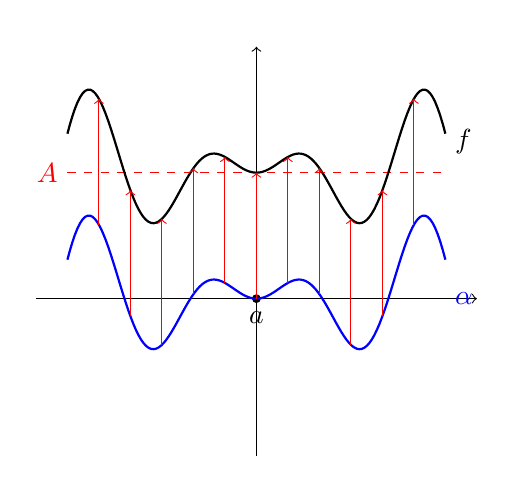
\begin{tikzpicture}[scale=0.8]
          % Coordinate axes
          \draw[->] (-3.5,0) -- (3.5,0) node[right] {};
          \draw[->] (0,-2.5) -- (0,4) node[above] {};
          
          % Point a on x-axis
          \node at (0,-0.3) {$a$};
          \fill (0,0) circle (0.07);
          
          % Blue function (alpha): x*sin(x)
          \draw[blue, thick, domain=-3:3, samples=150] 
            plot (\x, {0.5*\x*sin(3*\x r)});
          
          % Blue alpha label without arrow
          \node[blue, right] at (3,0) {$\alpha$};
          
          % Red horizontal line for A
          \draw[red, dashed] (-3,2) -- (3,2);
          \node[red, left] at (-3,2) {$A$};
          
          % Black function (f): x*sin(x) + 2
          \draw[black, thick, domain=-3:3, samples=150] 
            plot (\x, {0.5*\x*sin(3*\x r) + 2});
          
          % Black f label without arrow
          \node[black, right] at (3,2.5) {$f$};
          
          % Red vertical arrows connecting blue function to red line
          \foreach \x in {-2.5, -2.0, -1.5, -1.0, -0.5, 0, 0.5, 1.0, 1.5, 2.0, 2.5}
          \draw[->, red] (\x, {0.5*\x*sin(3*\x r)}) -- (\x, {0.5*\x*sin(3*\x r) + 2});
      \end{tikzpicture}
      \caption{Shift of $f(x) = \frac{1}{2} x \sin(3x) + 2$.} 
      \label{fig:infinitesimal_shift_function}
    \end{figure}
  \end{theorem}

  Finally, we reiterate some limit theorems already stated for sequences, but now corresponding to functions. Interpreting the function limit as the Cauchy sequence definition of limits renders the proofs of these theorems trivial. 

  \begin{theorem}[Bounds on Limits of Functions]
    If the functions $f, g: E \rightarrow \mathbb{R}$ are such that
    \begin{equation}
      \lim_{x\rightarrow a} f(x) = A < B = \lim_{x \rightarrow a} g(x)
    \end{equation}
    then there exists a deleted neighborhood $U_\delta (a)$ in $E$ at each point of which $f(x) < g(x)$. 
  \end{theorem}

  \begin{theorem}[Squeeze Theorem for Limits of Functions]
    Given the functions $f, g, h: E \subset \mathbb{R} \longrightarrow \mathbb{R}$ such that
    \begin{equation}
      f(x) \leq g(x) \leq h(x) \text{ for all } x \in E
    \end{equation}
    then, 
    \begin{equation}
      \lim_{x \rightarrow a} f(x) = \lim_{x \rightarrow a} h(x) = C \implies \lim_{x \rightarrow a} g(x) = C
    \end{equation}
  \end{theorem}

\subsection{Asymptotic Behavior of Functions}

    \begin{definition}[Little-O Notation]
      The function $f: E \longrightarrow \mathbb{R}$ is said to be \textbf{infinitesimal compared with the function $g: E \longrightarrow \mathbb{R}$} as $x \rightarrow a$, written (by abuse of notation) $f = o(g)$ as $x \rightarrow a$, if 
      \[\lim_{x \rightarrow a} \frac{f(x)}{g(x)} = 1\]
      or in other words, if $f/g$ is an infinitesimal function as $x \rightarrow a$. Therefore, $f = o(1)$ as $x \rightarrow a$ means that $f$ is infinitesimal as $x \rightarrow a$. \footnote{Note that writing $f = o(g)$ is again, an abuse of notation. $f = o(g)$ is really a shorthand way of writing that $f$ is in the class of functions that is infinitesimal compared with the function $g$.}
    \end{definition}

    Intuitively, $f = o(g)$ means that the ratio between $f(x)$ and $g(x)$ will tend to infinity as $x \rightarrow a$ (this does not mean that $f$ will be infinitely greater than $g$, however!). 

    \begin{example}[Linear vs Quadratic]
      For example, looking at the two functions $f(x) = x^2$ and $g(x) = x$, we have 
      \begin{enumerate}
        \item $x^2 = o(x)$ as $x \rightarrow 0$ (since $\frac{x^2}{x} = x$ is infinitesimal as $x \rightarrow 0$)
        \item $x = o(x^2)$ as $x \rightarrow \infty$ (since $\frac{x}{x^2} = \frac{1}{x}$ is infinitesimal as $x \rightarrow \infty$)
      \end{enumerate}
      We can visualize $g/f (x)$ tending to infinity within a neighborhood of $0$ and $f/g (x)$ tending to infinity within a neighborhood of $\infty$. 
      
      \begin{figure}[H]
        \centering 
        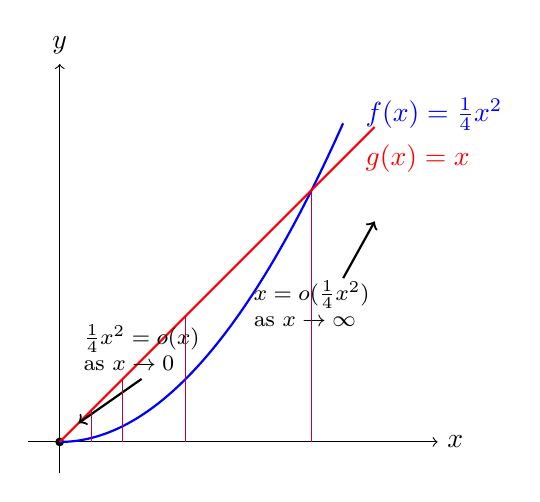
\begin{tikzpicture}[scale=0.8]
            % Coordinate axes
            \draw[->] (-0.5,0) -- (6,0) node[right] {$x$};
            \draw[->] (0,-0.5) -- (0,6) node[above] {$y$};
            
            % Origin point
            \fill (0,0) circle (0.07);
            
            % Blue parabola: f(x) = 1/4 * x^2
            \draw[blue, thick, domain=0:4.5, samples=100] 
              plot (\x, {0.25*\x*\x});
            
            % Red linear function: g(x) = x
            \draw[red, thick, domain=0:5, samples=2] 
              plot (\x, {\x});
            
            % Function labels
            \node[blue, right] at (4.7,5.2) {$f(x)=\frac{1}{4}x^2$};
            \node[red, right] at (4.7,4.5) {$g(x)=x$};
            
            % Asymptotic behavior annotations
            \node[align=left, font=\footnotesize] at (1.3,1.5) {$\frac{1}{4}x^2=o(x)$\\as $x\to 0$};
            \draw[->, thick] (1.3,1) -- (0.3,0.3);
            
            \node[align=left, font=\footnotesize] at (4,2.2) {$x=o(\frac{1}{4}x^2)$\\as $x\to\infty$};
            \draw[->, thick] (4.5,2.6) -- (5,3.5);
            
            % Vertical comparison lines
            \draw[purple, thin] (0.5,0) -- (0.5,0.5);
            \draw[purple, thin] (0.5,0) -- (0.5,0.0625);
            
            \draw[purple, thin] (1,0) -- (1,1);
            \draw[purple, thin] (1,0) -- (1,0.25);
            
            \draw[purple, thin] (2,0) -- (2,2);
            \draw[purple, thin] (2,0) -- (2,1);
            
            \draw[purple, thin] (4,0) -- (4,4);
            \draw[purple, thin] (4,0) -- (4,4);
        \end{tikzpicture}
        \caption{} 
        \label{fig:quadratic_vs_linear}
      \end{figure}
    \end{example}

    \begin{definition}[Orders of Infinitesimals, Infinities]
      If $f = o(g)$ and $g$ is infinitesimal as $x \rightarrow a$, then $f$ is an \textbf{infinitesimal of higher order than $g$ as $x \rightarrow a$}. Furthermore, if $f$ and $g$ are infinite functions as $x\rightarrow a$ and $f = o(g)$ as $x \rightarrow a$, then $g$ is a \textbf{higher order infinity than $f$ as $x \rightarrow a$}. 
    \end{definition}

    \begin{definition}[Big-O Notation]
      By abuse of notation, $f = O(g)$ as $x \rightarrow a$ means that 
      \begin{equation}
        \lim_{x \rightarrow a} \frac{f(x)}{g(x)} = \infty
      \end{equation}
      or in other words, $f/g$ is ultimately bounded as $x \rightarrow a$. In particular, $f = O(1)$ as $x \rightarrow a$ means that $f$ is bounded within a certain neighborhood $U(a)$ of $a$. 
    \end{definition}

    \begin{definition}[Functions of Same Order]
      The functions $f$ and $g$ are of the same over as $x \rightarrow a$, written 
      \begin{equation}
        f \asymp g \text{ as } x \rightarrow a
      \end{equation}
      if $f = O(g)$ and $g = O(f)$ as $x \rightarrow a$. Intuitively, this means that the ratio between $f$ and $g$ within some deleted neighborhood of $a$ is finite. 

      Note that the condition that $f$ and $g$ be of the same order as $x \rightarrow a$ is (by definition of ultimately bounded functions) equivalent to the condition that there exist $c_1, c_2 > 0$ and an open neighborhood $U (a)$ such that the relations
      \begin{equation}
        c_1 |g(x)| \leq |f(x)| \leq c_2 |g(x)|
      \end{equation}
      is true for $x \in U(a)$. 
    \end{definition}

    \begin{definition}[Asymptotic Equivalence of Functions]
      For functions $f$ and $g$, if 
      \begin{equation}
        \lim_{x \rightarrow a} \frac{f(x)}{g(x)} = 1
      \end{equation}
      we say that \textbf{$f$ behaves asymptotically like $g$ as $x \rightarrow a$}, or that \textbf{$f$ is equivalent to $g$ as $x \rightarrow a$}, written 
      \begin{equation}
        f \sim g \text{ as } x \rightarrow a
      \end{equation}
      Moreover, $\sim$ is an equivalence relation, which means that
      \begin{enumerate}
        \item $f \sim f$ as $x \rightarrow a$
        \item $f \sim g$ as $x \rightarrow a \implies$ $g \sim f$ as $x \rightarrow a$
        \item $f \sim g$ and $g \sim h$ as $x \rightarrow a \implies f \sim h$ as $x \rightarrow a$
      \end{enumerate}
    \end{definition}

    We list a few examples in order to develop some sort of visual intuition for when two functions are asymptotically equivalent. 

    \begin{example}[Both Converges at Finite Value to Nonzero Finite Value]
      If $f(a) = g(a) \neq 0$, then $f \sim g$ trivially since the ratio of $f$ and $g$ converges to $1$ within a neighborhood of $a$. 

      \begin{figure}[H]
        \centering 
        \begin{tikzpicture}[scale=1.2]
          % Coordinate axes
          \draw[->] (-3,0) -- (3,0) node[right] {$x$};
          \draw[->] (0,-1) -- (0,3) node[above] {$y$};
          
          % Blue curve - single smooth wave with no other intersections
          \draw[blue, thick, smooth] 
            plot[domain=-3:3, samples=50] (\x, {1.5 + 0.8*sin(\x*40)});
          
          % Red curve - continuous rise with no other intersections
          \draw[red, thick, smooth] 
            plot[domain=-2:3, samples=50] (\x, {0.2*\x*\x - 0.6*\x + 1});
          
          % Point of intersection
          \fill (-0.4,1.25) circle (0.05);
          \node[above] at (-0.4,1.25) {$a$};
        \end{tikzpicture}
        \caption{} 
      \end{figure}
    \end{example}

    \begin{example}[Both Converges at Finite Value to $0$]
      When $f(a) = g(a) = 0$, it may be $f$ may be equivalent to $g$ or one function may be infinitesimally smaller than the other. 

      \begin{figure}[H]
        \centering
        \begin{subfigure}[b]{0.48\textwidth}
          \centering
          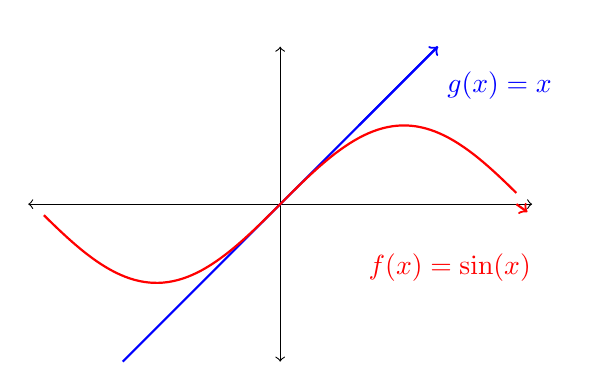
\begin{tikzpicture}[scale=1.0]
            % Coordinate axes
            \draw[<->] (-3.2,0) -- (3.2,0) node[right] {};
            \draw[<->] (0,-2) -- (0,2) node[above] {};
            
            % Blue line g(x) = x with restricted domain
            \draw[blue, thick] (-2,-2) -- (2,2);
            \node[blue, right] at (2,1.5) {$g(x)=x$};
            
            % Red sine curve f(x) = sin(x)
            \draw[red, thick, domain=-3:3, samples=100] 
              plot (\x, {sin(\x r)});
            \node[red, right] at (1,-0.8) {$f(x)=\sin(x)$};
            
            % Direction arrows
            \draw[blue, ->, thick] (1,1) -- (2,2);
            \draw[red, ->, thick] (3,0) -- (3.14,-0.1);
          \end{tikzpicture}
          \caption{When $f(x) = \sin{x}$ and $g(x) = x$, then $f \sim g$ since we see that $\lim_{x \rightarrow 0} \frac{\sin{x}}{x} = 1$, and so $\sin{x} \sim x$ as $x \rightarrow 1$. }
        \end{subfigure}
        \hfill 
        \begin{subfigure}[b]{0.48\textwidth}
          \centering
          \begin{tikzpicture}[scale=0.8]
            % Coordinate axes
            \draw[<->] (-3.5,0) -- (3.5,0) node[right] {};
            \draw[<->] (0,-3) -- (0,3) node[above] {};
            
            % Red parabola f(x) = x^2
            \draw[red, thick, domain=-2.5:2.5, samples=50] 
              plot (\x, {\x*\x*0.2});
            \node[red, right] at (2.5,2.5) {$f(x)=x^2$};
            
            % Blue cubic g(x) = x^3
            \draw[blue, thick, domain=-2.3:2.3, samples=50] 
              plot (\x, {\x*\x*\x*0.2});
            \node[blue, right] at (2.5,2) {$g(x)=x^3$};
          \end{tikzpicture}
          \caption{When $f(x) = x^2$ and $g(x) = x^3$, then $\lim_{x \rightarrow 0} \frac{x^3}{x^2} = 0$, and so $x^3 \not\sim x^2$. In fact, $x^3 = o(x^2)$. }
        \end{subfigure}

        \begin{subfigure}[b]{0.48\textwidth}
          \centering
          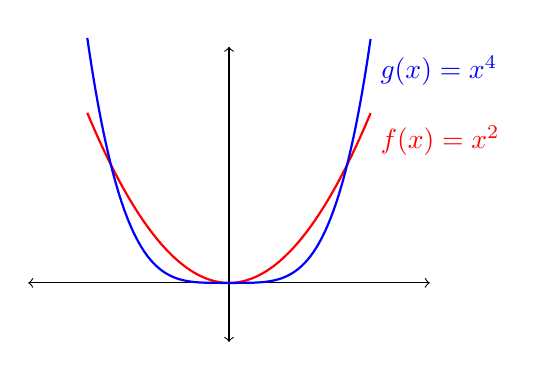
\begin{tikzpicture}[scale=1.5]
            % Coordinate axes
            \draw[<->] (-1.7,0) -- (1.7,0) node[right] {};
            \draw[<->] (0,-0.5) -- (0,2) node[above] {};
            
            % Red parabola f(x) = x^2
            \draw[red, thick, domain=-1.2:1.2, samples=100] 
              plot (\x, {\x*\x});
            \node[red, right] at (1.2,1.2) {$f(x)=x^2$};
            
            % Blue g(x) = x^4
            \draw[blue, thick, domain=-1.2:1.2, samples=100] 
              plot (\x, {\x*\x*\x*\x});
            \node[blue, right] at (1.2,1.8) {$g(x)=x^4$};
          \end{tikzpicture}
          \caption{When $f(x) = x^2$ and $g(x) = x^4$, then  $\lim_{x \rightarrow 0} \frac{x^4}{x^2} = 0$, and so $x^4 \not\sim x^2$. In fact, $x^4 = o(x^2)$. }
        \end{subfigure}
        \hfill 
        \begin{subfigure}[b]{0.48\textwidth}
          \centering
          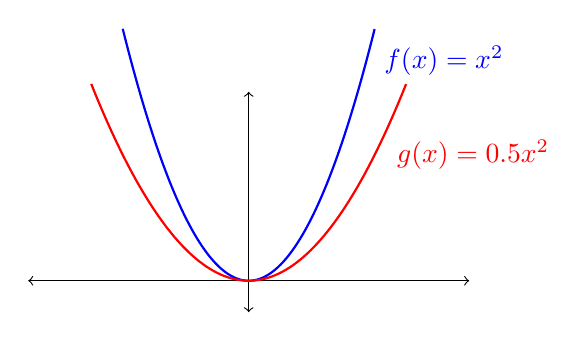
\begin{tikzpicture}[scale=0.8]
            % Coordinate axes
            \draw[<->] (-3.5,0) -- (3.5,0) node[right] {};
            \draw[<->] (0,-0.5) -- (0,3) node[above] {};
            
            % Blue parabola f(x) = x^2
            \draw[blue, thick, domain=-2:2, samples=100] 
              plot (\x, {\x*\x});
            \node[blue, right] at (2,3.5) {$f(x)=x^2$};
            
            % Red parabola g(x) = 0.5x^2
            \draw[red, thick, domain=-2.5:2.5, samples=100] 
              plot (\x, {0.5*\x*\x});
            \node[red, right] at (2.2,2) {$g(x)=0.5x^2$};
          \end{tikzpicture}
          \caption{When $f(x), g(x) = x^2, 0.5x^2$, then $\lim_{x \rightarrow 0} \frac{0.5x^2}{x^2} = \frac{1}{2}$. So $0.5x^2 \not\sim x^2$. }
        \end{subfigure}
        \caption{Examples of different scenarios.}
        \label{fig:converge_to_finite_value_0}
      \end{figure}
    \end{example}

    \begin{example}[Analyzing at Infinity]
      When analyzing the behavior of functions as $x \rightarrow \infty$, we can picture the two graphs of $f$ and $g$ on the plane and "zoom out" to see if the ratio of the values converge to $1$. This would mean that as $x \rightarrow \infty$, we should see the graphs overlapping more and more. 

      \begin{figure}[H]
        \centering
        \begin{subfigure}[b]{0.48\textwidth}
          \centering
          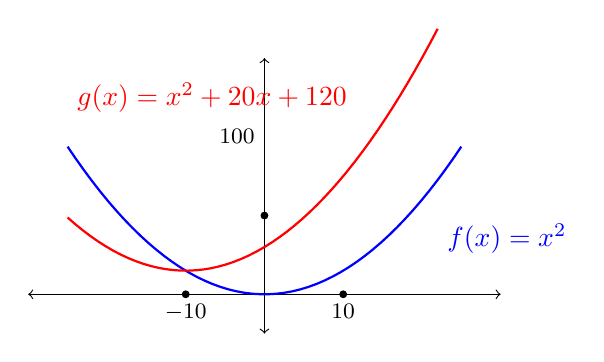
\begin{tikzpicture}[scale=1]
              % Coordinate axes
              \draw[<->] (-3,0) -- (3,0) node[right] {};
              \draw[<->] (0,-0.5) -- (0,3) node[above] {};
              
              % Blue parabola f(x) = x^2
              \draw[blue, thick, domain=-2.5:2.5, samples=50] 
                plot (\x, {0.3 * \x*\x});
              \node[blue, right] at (2.2,0.7) {$f(x)=x^2$};
              
              % Red parabola g(x) = x^2 + 10x + 100
              \draw[red, thick, domain=-2.5:2.2, samples=50] 
                plot (\x, {0.3 * (\x*\x + 2*\x + 2)});
              \node[red, right] at (-2.5,2.5) {$g(x)=x^2+20x+120$};
              
              % Key points on x-axis with labels
              \fill (-1,0) circle (0.05);
              \node[below, font=\footnotesize] at (-1,0) {$-10$};
              
              \fill (1,0) circle (0.05);
              \node[below, font=\footnotesize] at (1,0) {$10$};
              
              \fill (0,1) circle (0.05);
              \node[left, font=\footnotesize] at (0,2) {$100$};
          \end{tikzpicture}
          \caption{Comparison of $f(x)=x^2$ and $g(x)=x^2+10x+100$}
          \label{fig:shifted-quadratic}
        \end{subfigure}
        \hfill 
        \begin{subfigure}[b]{0.48\textwidth}
          \centering
          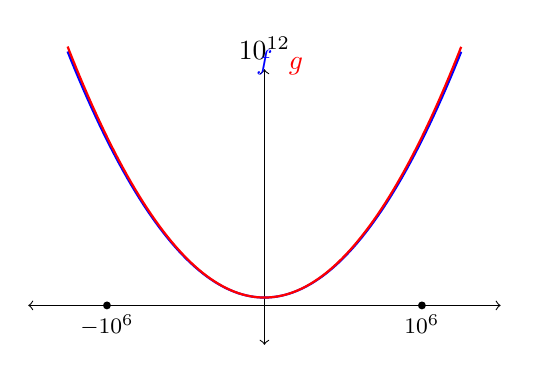
\begin{tikzpicture}[scale=1]
              % Coordinate axes
              \draw[<->] (-3,0) -- (3,0) node[right] {};
              \draw[<->] (0,-0.5) -- (0,3) node[above] {$10^{12}$};
              
              % Functions with nearly identical behavior
              \draw[blue, thick, domain=-2.5:2.5, samples=100] 
                plot (\x, {0.1 + 0.5*\x*\x});
              \node[blue, above] at (0,2.8) {$f$};
              
              % Red function slightly above blue
              \draw[red, thick, domain=-2.5:2.5, samples=100] 
                plot (\x, {0.1 + 0.51*\x*\x});
              \node[red, above] at (0.4,2.8) {$g$};
              
              % Key points on x-axis with labels
              \fill (-2,0) circle (0.05);
              \node[below, font=\footnotesize] at (-2,0) {$-10^6$};
              
              \fill (2,0) circle (0.05);
              \node[below, font=\footnotesize] at (2,0) {$10^6$};
          \end{tikzpicture}
          \caption{Asymptotic behavior with $g/f \approx 1$}
          \label{fig:asymptotic}
        \end{subfigure}
        \caption{taking $f(x) = x^2$ and $g(x) = x^2 + 10x + 100$, we can see that the discrepancy is high around a neighborhood of $x = 0$. But as $x \rightarrow +\infty$, we get $\lim_{x \rightarrow + \infty} \frac{x^2 + 10x + 100}{x^2} = 1$, and so the graphs look like they are overlapping. Notice that even though the absolute difference $|(x^2 + 10x + 100) - x^2| = |10x + 100|$ tends to infinity, this difference increases infinitesimally compared to $f$ and $g$. }
        \label{fig:function-ratios}
      \end{figure}
    \end{example}

    From this, we can see that if $f \sim g$ as $x \rightarrow a$, then their difference 
    \begin{equation}
      f - g = o(g) = o(f)
    \end{equation}
    That is, $(f-g)(x)$ is infinitesimal compared to $g$ or $f$ (doesn't matter which one we compare it to). This leads to our next section, where we formalize this concept with absolute and relative errors. 

  \subsubsection{Approximations of Functions}

    It is useful to note that since the relation $\lim_{x \rightarrow a} \gamma(x) = 1$ is equivalent to 
    \begin{equation}
      \gamma (x) = 1 + \alpha(x), \text{ where } \lim_{x \rightarrow a} \alpha(x) = 0
    \end{equation}
    the relation $f \sim g$ as $x\rightarrow a$ is equivalent to saying that
    \begin{equation}
      \frac{f(x)}{g(x)} = \gamma(x), \text{ where } \lim_{x \rightarrow a} \gamma(x) = 1
    \end{equation}
    which implies 
    \begin{equation}
      f(x) = g(x) + \alpha(x) g(x) = g(x) + o(g(x)) \text{ as } x \rightarrow a
    \end{equation}
    or, symmetrically, 
    \begin{equation}
      g(x) = f(x) + \alpha(x) f(x) = f(x) + o(f(x)) \text{ as } x \rightarrow a
    \end{equation}
    This means that $f$ can be exactly represented by another function $g$, plus another (error) function $o(g(x))$ that is infinitesimal compared to $g$. 

    \begin{figure}[H]
      \centering
      \begin{subfigure}[b]{0.48\textwidth}
        \centering
        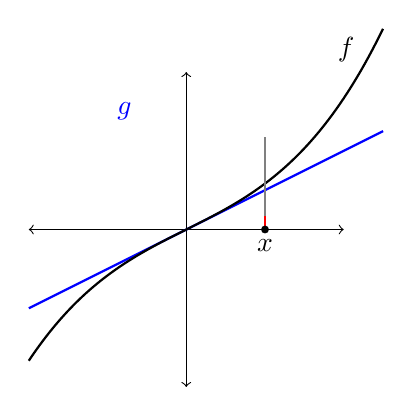
\begin{tikzpicture}[scale=1]
            % Coordinate axes
            \draw[<->] (-2,0) -- (2,0) node[right] {};
            \draw[<->] (0,-2) -- (0,2) node[above] {};
            
            % Blue line g(x) = x
            \draw[blue, thick, domain=-2:2.5, samples=2] 
              plot (\x, {\x * 0.5});
            \node[blue, right] at (-1,1.5) {$g$};
            
            % Black cubic f(x) = x^3/6 + x
            \draw[black, thick, domain=-2:2.5, samples=100] 
              plot (\x, {((\x*\x*\x)/6 + \x) * 0.5});
            \node[black, above right] at (1.8,2) {$f$};
            
            % Vertical line at a point
            \draw[gray, thin] (1,0) -- (1,1);
            \draw[gray, thin] (1,1) -- (1,1.17);
            \draw[red, thin] (1,0) -- (1,0.17);
            
            % Point label
            \fill (1,0) circle (0.05);
            \node[below] at (1,0) {$x$};
        \end{tikzpicture}
        \caption{Functions $f$, $g$, and their difference}
        \label{fig:function-diff}
      \end{subfigure}
      \hfill 
      \begin{subfigure}[b]{0.48\textwidth}
        \centering
        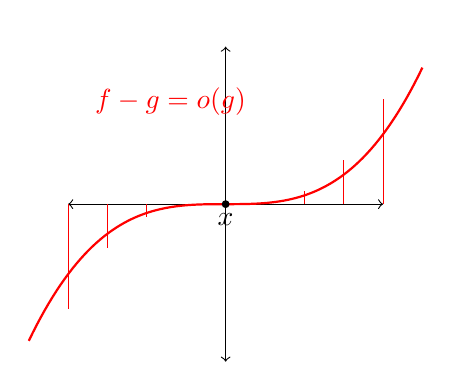
\begin{tikzpicture}[scale=1]
            % Coordinate axes
            \draw[<->] (-2,0) -- (2,0) node[right] {};
            \draw[<->] (0,-2) -- (0,2) node[above] {};
            
            % Red function f-g = x^3/6
            \draw[red, thick, domain=-2.5:2.5, samples=100] 
              plot (\x, {(\x*\x*\x)/9});
            \node[red, above] at (-0.7,1) {$f-g = o(g)$};
            
            % Vertical lines showing difference
            \foreach \x in {-2, -1.5, -1, -0.5, 0.5, 1, 1.5, 2} {
                \draw[red, thin] (\x,0) -- (\x,{(\x*\x*\x)/6});
            }
            
            % Point at origin
            \fill (0,0) circle (0.05);
            \node[below] at (0,0) {$x$};
        \end{tikzpicture}
        \caption{Behavior of $f-g$ (little-o of $g$)}
        \label{fig:little-o}
      \end{subfigure}
      \caption{Visualization of asymptotic behavior where $f-g = o(g)$}
      \label{fig:asymptotic-behavior}
    \end{figure}

    Note that it is not a sufficient condition that the error function be infinitesimal! The error function $f-g$ must be infinitesimal \textit{compared to $g$}! This tells us that not only does the error function decrease infinitesimally, but also is infinitesimal compared to the approximation function we already have, which is in general a much stronger claim. This representation of certain types functions will provide the foundation for differential calculus when we talk about "good" approximations for a function. 


    \begin{definition}[Relative Error]
      Since $f \sim g$ as $x \rightarrow a$ means that 
      \begin{equation}
        f(x) = g(x) + \alpha(x) g(x) = g(x) + o(g(x))
      \end{equation}
      we can define the \textbf{relative error} of $g$ as an approximation of $f$ to be
      \begin{equation}
        |\alpha(x)| = \bigg| \frac{f(x) - g(x)}{g(x)} \bigg|
      \end{equation}
      Clearly, since $f \sim g$, the relative error must be infinitesimal as $x \rightarrow a$. 
    \end{definition}

    We use the following lemma to check whether two functions are asymptotically equivalent. 
    \begin{lemma}
      $f \sim g$ as $x \rightarrow a$ if and only if the relative error of $g$ is infinitesimal as $x \rightarrow a$. 
    \end{lemma}

    \begin{example}
      We claim that 
      \begin{equation}
        x^2 + x = \bigg(1 + \frac{1}{x} \bigg) x^2 \sim x^2 \text{ as } x \rightarrow \infty
      \end{equation}
      We see that the absolute error of this approximation $|(x^2 + x) - x^2| = |x|$ tends to infinity, but the relative error $\frac{|x|}{x^2} = \frac{1}{|x|} \rightarrow 0$ as $x \rightarrow \infty$. 
    \end{example}

    \begin{theorem}[Prime Number Theorem]
      Let $\pi(x)$ be the number of prime numbers strictly less than $x$. Then $\pi \sim \frac{x}{\ln{x}}$ as $x\rightarrow + \infty$, or more precisely, 
      \begin{equation}
        \pi(x) = \frac{x}{\ln{x}} + o \bigg( \frac{x}{\ln{x}}\bigg) \text{ as } x \rightarrow +\infty
      \end{equation}
    \end{theorem}

    \begin{example}
      It is a fact that $\lim_{x\rightarrow 0} \frac{sin{x}}{x} = 1$, so we have $\sin{x} \sim x$ as $x \rightarrow 0$. So,
      \begin{equation}
        \sin{x} = x + o(x) \text{ as } x \rightarrow 0
      \end{equation}
    \end{example}

    The following theorem proves useful when computing limits. 

    \begin{theorem}
      If $f \sim \Tilde{f}$ as $x \rightarrow a$, then 
      \begin{equation}
        \lim_{x \rightarrow a} f(x) g(x) = \lim_{x \rightarrow a} \Tilde{f}(x) g(x)
      \end{equation}
      provided one of these limits exist. 
    \end{theorem}

    \begin{theorem}[Properties of $o(g)$ and $O(g)$ Functions]
      For $x \rightarrow a$, 
      \begin{enumerate}
        \item $o(f) + o(f) = o(f)$
        \item $o(f)$ is also $O(f)$
        \item $o(f) + O(f) = O(f)$
        \item $O(f) + O(f) = O(f)$
        \item If $g(x) \not\equiv 0$, then 
        \begin{equation}
          \frac{o(f(x))}{g(x)} = o \bigg( \frac{f(x)}{g(x)} \bigg), \text{ and } \frac{O(f(x))}{g(x)} = O \bigg( \frac{f(x)}{g(x)} \bigg)
        \end{equation}
      \end{enumerate}
    \end{theorem}

\subsection{Continuous Functions}

  \begin{definition}[Continuity of a Function]
    A function $f$ is \textbf{continuous at point $a$} if for any neighborhood $V\big(f(a)\big)$ of $f(a)$, there is a neighborhood $U(a)$ of $a$ whose image under the mapping $f$ is contained in $V\big( f(a)\big)$. 

    Generalizing this, we say that a function is \textbf{(globally) continuous} if the preimage of every neighborhood in its codomain is an open set in its domain. 
  \end{definition}

  \begin{lemma}[Existence of Limits of Continuous Functions]
    $f: E \longrightarrow \mathbb{R}$ is continuous at $a \in E$, where $a$ is a limit point of $E$ if and only if 
    \begin{equation}
      \lim_{x \rightarrow a} f(x) = f(a)
    \end{equation}
  \end{lemma}
  \begin{proof}
    The limit equaling $f(a)$ means that, by definition, for any arbitrarily small deleted neighborhood of $f(a)$, denoted $U_{f(a)} \setminus f(a)$, its preimage will be an open neighborhood of $a$, which itself will contain an open set. 
  \end{proof}

  This also means that we can use the Cauchy limit definition to defined continuity of a function at a point. That is, for any sequence $\{a_n\}$ of point in codomain $E$ which converges to point $a$, the function $f$ is continuous at $a$ if the corresponding sequence $\{f(a_n)\}$ converges to $f(a)$.

  \begin{theorem}
    This means that the continuous functions commute with the operation of passing to the limit at a point. 
    \begin{equation}
      \lim_{x \rightarrow a} f(x) = f\Big( \lim_{x \rightarrow a} x \Big)
    \end{equation}
  \end{theorem}

  \begin{lemma}[Properties of Continuous Functions]
    Let $f: \mathbb{R}^n \longrightarrow \mathbb{R}^m, \; g: \mathbb{R}^m \longrightarrow \mathbb{R}^p$ with $c \in \mathbb{R}$. 
    \begin{enumerate}
      \item $f$ continuous at $x_0 \implies$ $c f$ continous at $x_0$. 
      \item $f, g$ continuous at $x_0 \implies f + g$ continuous at $x_0$. 
      \item Let $m = 1$. $f, g$ continuous at $x_0 \implies f g$ continuous at $x_0$. 
      \item $f$ continuous at $x_0$ and $f(x) \neq 0 \forall x \in \mathbb{R}^n \implies 1 / f$ continuous at $x_0$. 
      \item If $f(x) = \big( f_1(x), f_2(x), ..., f_n(x) \big)$ coordinate-wise, then 
      \begin{equation}
        f \text{ continuous at } x_0 \iff f_1, f_2, ..., f_m \text{ continuous  at } x_0
      \end{equation}
      \item $f$ continuous at $x_0$ and $g$ continuous at $y_0 = f(x_0) \implies g \circ f$ continuous at $x_0$. 
    \end{enumerate}
  \end{lemma}
  \begin{proof}
    This is an immediate result of the equivalence of a function being continuous at point $a$ and its limit at point $a$ existing. 
  \end{proof}

  \begin{theorem}[Local Properties of Continuous Functions]
    Let $f: E \longrightarrow \mathbb{R}$ be a function that is continuous at the point $a \in E$. Then, 
    \begin{enumerate}
      \item $f$ is bounded in some neighborhood $U(a)$. 
      \item If $f(a) \neq 0$, then in some neighborhood $U(a)$ all the values of the function have the same sign as $f(a)$. 
      \item If the function $g: U(a) \subset E \longrightarrow \mathbb{R}$ is defined in some neighborhood of $a$ and is continuous at $a$, then the following functions 
      \begin{align*}
        & (f + g) (x) \\
        & (f \cdot g) (x) \\
        & \bigg( \frac{f}{g} \bigg) \big( x \big) \text{ where } g(a) \neq 0
      \end{align*}
      are also defined in $U(a)$ and continuous at $a$. 
      \item If the function $g: Y \longrightarrow \mathbb{R}$ is continuous at a point $b \in Y$ and $f$ is such that $f: E \longrightarrow Y$, $f(a) = b$, and $f$ is continuous at $a$, then the composite function 
      \[g \circ f: E \longrightarrow \mathbb{R}\]
      is defined on $E$ and continuous at $a$. This is easy to see because given the open neighborhood of $g(b)$, we know for a fact that $U_\delta (a)$ maps completely into $U_\epsilon (b)$, and that $U_\epsilon (b)$ maps completely into $U_\kappa (g(b))$ and so the composition of these mappings must mean that $U_\delta (a)$ maps completely into $U_\kappa (g(b))$. 
    \end{enumerate}
  \end{theorem}

  \begin{example}
    An algebraic polynomial 
    \begin{equation}
      P(x) = a_0 x^n + a_1 x^{n-1} + a_2 x^{n-2} + \ldots + a_{n-1} x + a_n
    \end{equation}
    is a continuous function on $\mathbb{R}$. Since $f(x) = x$ and $f(x) = c$ are continuous functions, by induction on $x$, we can multiply them together to find that $f(x) = x^n$ is continuous, which implies that $a x^n$ is continuous, which implies that the sums of these functions are also continuous. 
  \end{example}

  \subsubsection{Intermediate and Extreme Value Theorem}

    Unlike local properties, the global property of a function is a property involving the entire domain of definition of the function. 

    \begin{theorem}[Compact Sets to Compact]
      If $f: X \rightarrow Y$ is continuous and $K \subset X$ is compact, then $f(K)$ is compact in $Y$. 
    \end{theorem}
    \begin{proof}
      
    \end{proof}

    \begin{corollary}[Extreme Value Theorem]
      A continuous real-valued function over a compact set attains its maximum and minimum. 
    \end{corollary}

    \begin{theorem}[Intermediate Value Theorem]
      If a function $f$ is continuous on an open interval and assumes values $f(a) = A, f(b) = B$, then for any number $C \in (A, B)$, there is a point $c$ between $a$ and $b$ such that $f(c) = C$. 

      \begin{figure}[H]
        \centering 
        \begin{tikzpicture}[scale=1]
          % Draw the coordinate axes
          \draw[->] (-1.5,0) -- (5,0) node[right] {};
          \draw[->] (0,-3) -- (0,3) node[above] {};
          
          % Draw the continuous function curve
          \draw[thick] (-1,-2) to[out=40,in=180] (1,-2.3) 
            to[out=0,in=240] (3,0) 
            to[out=60,in=240] (4,2);
          
          % Draw the interval [a,b] on the x-axis with blue color
          \draw[blue, thick] (-1,0) -- (4,0);
          
          % Mark points a, c, and b
          \draw[blue] (-1,0.1) -- (-1,-0.1) node[below] {$a$};
          \draw[blue] (2.7,0.1) -- (2.7,-0.1) node[below] {$c$};
          \draw[blue] (4,0.1) -- (4,-0.1) node[below] {$b$};
          \draw[red] (-0.1,2) -- (0.1,2) node[left] {$f(a)$};
          \draw[red] (-0.1,-2) -- (0.1,-2) node[left] {$f(b)$};
          \draw[red] (-0.1,-0.5) -- (0.1,-0.5) node[left] {$f(c)$};

          \draw[fill] (2.7,-0.6) circle (0.05) node[left] {};
          \draw[fill] (-1,-2) circle (0.05) node[left] {};
          \draw[fill] (4,2) circle (0.05) node[left] {};
          
          % Add the f label without an arrow
          \node at (3,1) {$f$};
        \end{tikzpicture}
        \caption{Illustration of a continuous function with a root in the interval $[a,b]$}
        \label{fig:continuous-function-root}
      \end{figure}
    \end{theorem}
    \begin{proof}

    \end{proof}

    This following proof provides a very simple algorithm for finding the zero of the equation $f(x) = 0$ on an interval whose endpoints has values with opposite signs. 
    Note that the colloquial description of the intermediate value theorem, that is is impossible to pass continuously from positive to negative values without assuming the value $0$ along the way), assumes more than they state. That is, this theorem is actually dependent on the domain of definition: that is is a closed interval, or more generally, that it is \textbf{connected}. 


  \subsubsection{Inverse Function Theorem}

    We begin by introducing this intuitive lemma. 
    \begin{lemma}
      A continuous mapping $f: E \longrightarrow \mathbb{R}$ of a closed interval $E = [a,b]$ into $\mathbb{R}$ is injective if and only if the function $f$ is strictly monotonic on $[a,b]$. 

      Furthermore, every strictly monotonic function $f: X \subset \mathbb{R} \longrightarrow \mathbb{R}$ (for arbitrary $X$) has an inverse 
      \[f^{-1}: f(X) \subset \mathbb{R} \longrightarrow \mathbb{R}\]
      with the same kind of monotonicity on $f(X)$ that $f$ has on $X$. 
    \end{lemma}

    \begin{lemma}[Criterion for Continuity of a Monotonic Function]
      A monotonic function $f: E \longrightarrow \mathbb{R}$ defined on a closed interval $E = [a,b]$ is continuous if and only if its set of values $f(E)$ is the closed interval with endpoints $f(a)$ and $f(b)$. 

      Note that both conditions imply that there are no points of discontinuities in the graph of $f$. 
    \end{lemma}


    \begin{theorem}[Inverse Function Theorem]
    A function $f: X \longrightarrow \mathbb{R}$ that is strictly monotonic on a set $X \subset \mathbb{R}$ has an inverse $f^{-1}: Y \longrightarrow \mathbb{R}$ defined on the set $Y = f(X)$ of values of $f$. The function $f^{-1}: Y \longrightarrow \mathbb{R}$ is monotonic and has the same type of monotonicity on $Y$ that $f$ has on $X$. 
    \begin{center}
        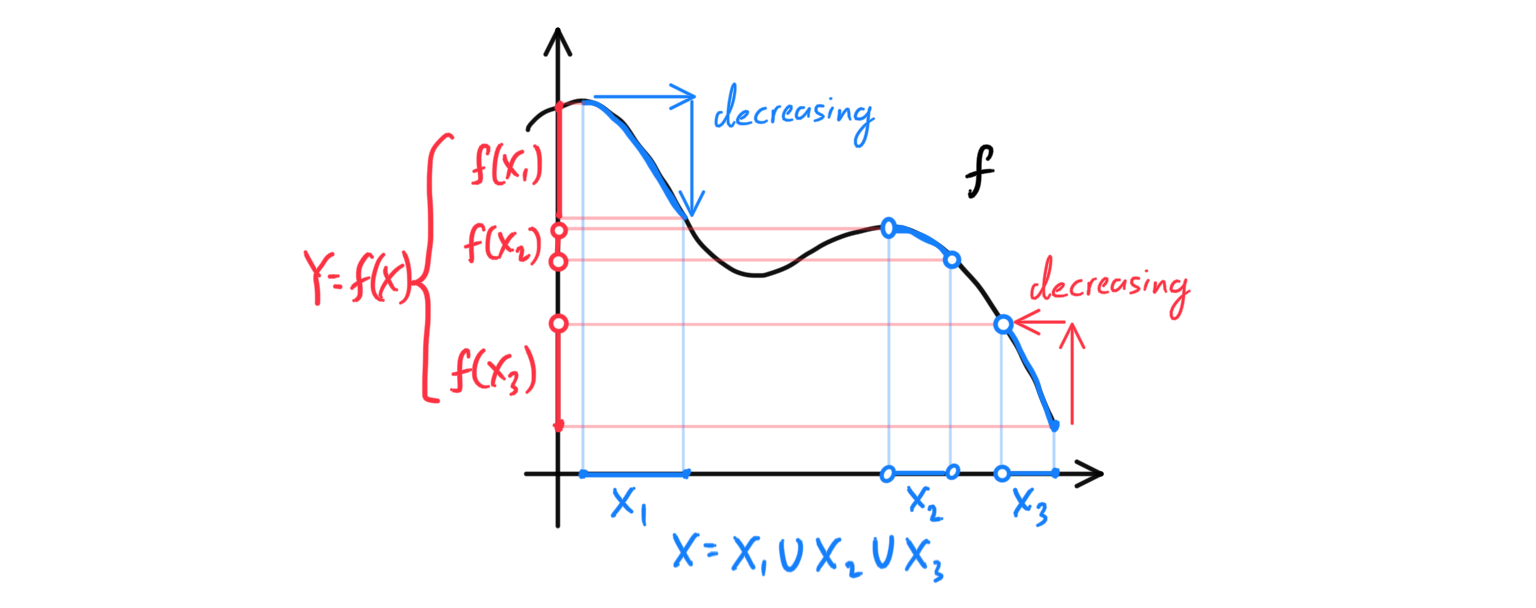
\includegraphics[scale=0.25]{img/Inverse_Function_Theorem_Analysis.PNG}
    \end{center}
    If in addition, $X$ is a closed interval $[a,b]$ and $f$ is continuous on $X$, then the set $Y = f(X)$ is the closed interval with endpoints $f(a)$ and $f(b)$ and the function $f^{-1}: Y \longrightarrow \mathbb{R}$ is continuous on it.
    \end{theorem}

    \begin{example}[Sin and Arcsin]
      The function $f(x) = \sin{x}$ is increasing and continuous on the closed interval $\big[ -\frac{\pi}{2}, \frac{\pi}{2} \big]$. Hence, the restriction to the closed interval $\big[ -\frac{\pi}{2}, \frac{\pi}{2} \big]$ has an inverse $x = f^{-1}(y)$, called the \textbf{arcsin}, and denoted by $x = \arcsin{y}$.

      \begin{figure}[H]
        \centering 
        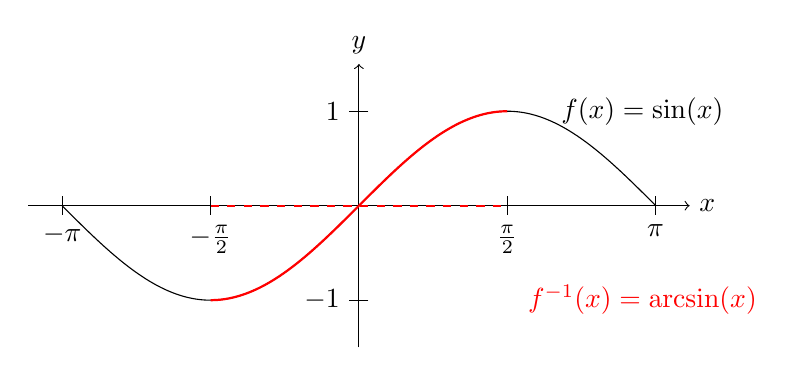
\begin{tikzpicture}[scale=1.2]
          % Draw the coordinate axes
          \draw[->] (-3.5,0) -- (3.5,0) node[right] {$x$};
          \draw[->] (0,-1.5) -- (0,1.5) node[above] {$y$};
          \draw[-, thick, red, dashed] (-1.57, 0) -- (1.57, 0) node[above] {};
          
          % Draw the full sine curve in black
          \draw[samples=100, smooth] plot[domain=-3.14:3.14] (\x, {sin(\x r)});
          
          % Draw the partial sine curve in thicker blue
          \draw[thick, red, samples=50, smooth] plot[domain=-1.57:1.57] (\x, {sin(\x r)});
          
          % Add tick marks and labels for key points
          \draw (-3.14,0.1) -- (-3.14,-0.1) node[below] {$-\pi$};
          \draw (-1.57,0.1) -- (-1.57,-0.1) node[below] {$-\frac{\pi}{2}$};
          \draw (1.57,0.1) -- (1.57,-0.1) node[below] {$\frac{\pi}{2}$};
          \draw (3.14,0.1) -- (3.14,-0.1) node[below] {$\pi$};
          
          \draw (0.1,-1) -- (-0.1,-1) node[left] {$-1$};
          \draw (0.1,1) -- (-0.1,1) node[left] {$1$};
          
          % Add function label
          \node at (3,1) {$f(x) = \sin(x)$};
          \node[red] at (3,-1) {$f^{-1}(x) = \arcsin(x)$};
        \end{tikzpicture}
        \caption{This function is defined on the closed interval $\big[- \sin\big(-\frac{\pi}{2}\big), \sin\big(-\frac{\pi}{2}\big) \big] = [-1,1]$ and increases continuously from $-\frac{\pi}{2}$ to $\frac{\pi}{2}$. } 
        \label{fig:sine-graph-highlight}
      \end{figure}
    \end{example}

\subsection{Uniform Continuity}

  Roughly speaking, a function $f$ is uniformly continuous if it is possible to guarantee that $f(x)$ and $f(y)$ be as close to each other as we please by requiring only that $x$ and $y$ be sufficiently close to each other. Intuitively, uniform continuity says that given any two points $x, y$ in the domain where their distance is arbitrarily small ($\delta$ apart), we can guarantee that the distance between $f(x), f(y)$ is at maximum some arbitrarily small $\epsilon$. 

  \begin{definition}[Uniform Continuity]
    A function $f: E \longrightarrow \mathbb{R}$ is \textbf{uniformly continuous} on a set $E \subset \mathbb{R}$ if for every $\epsilon > 0$, there exists $\delta > 0$ such that 
    \begin{equation}
      \big| f(x_1) - f(x_2)\big| < \epsilon
    \end{equation}
    for all points $x_1, x_2 \in E$ such that $|x_1 - x_2| < \delta$. 
  \end{definition}

  \begin{example}[Uniformly Continuous]
    The following visual shows the radical function $f(x) = \sqrt{x}$ defined on $\mathbb{R}^+$. We can see that it satisfies uniform continuity because the graph does not escape the top and/or bottom of the $\epsilon \times \delta$ window, no matter where the box is located on the graph. More strictly speaking, no matter what we set the $\epsilon$ (how long the box is), uniform continuity says that we can choose a sufficient $\delta$ (width of the box) such that the graph does not escape the top/bottom of the window no matter where the window is. 

    \begin{figure}[H]
      \centering 
      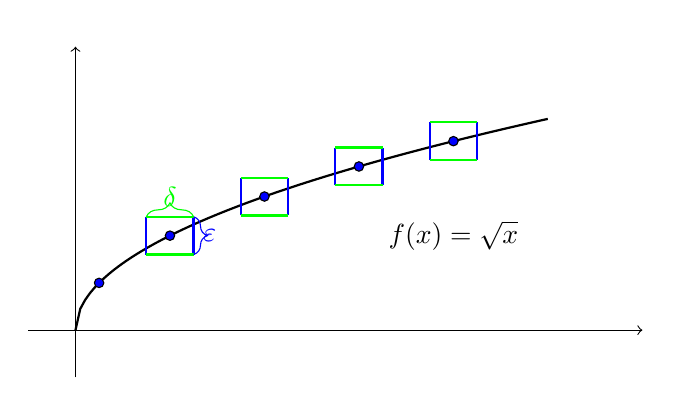
\begin{tikzpicture}[scale=1.2]
        % Draw the coordinate axes
        \draw[->] (-0.5,0) -- (6,0) node[right] {};
        \draw[->] (0,-0.5) -- (0,3) node[above] {};
        
        % Draw the square root curve
        \draw[thick] plot[domain=0:5, samples=100] (\x, {sqrt(\x)});
        
        % Draw points on the curve
        \foreach \x in {0.25, 1, 2, 3, 4} {
          \draw[fill=blue] (\x, {sqrt(\x)}) circle (0.05);
        }
        
        % Draw epsilon-delta boxes with consistent dimensions
        % Each box has same dimensions, with blue vertical edges and green horizontal edges
        \foreach \x in {1, 2, 3, 4} {
          % Calculate box coordinates
          \pgfmathsetmacro{\xmin}{\x - 0.25}
          \pgfmathsetmacro{\xmax}{\x + 0.25}
          \pgfmathsetmacro{\ymin}{sqrt(\x) - 0.2}
          \pgfmathsetmacro{\ymax}{sqrt(\x) + 0.2}
          
          % Draw left and right (vertical) edges in blue
          \draw[blue, thick] (\xmin, \ymin) -- (\xmin, \ymax);
          \draw[blue, thick] (\xmax, \ymin) -- (\xmax, \ymax);
          
          % Draw top and bottom (horizontal) edges in green
          \draw[green, thick] (\xmin, \ymin) -- (\xmax, \ymin);
          \draw[green, thick] (\xmin, \ymax) -- (\xmax, \ymax);
        }
        
        % Add function label
        \node at (4,1) {$f(x)=\sqrt{x}$};
        
        % Draw curly brace for epsilon (height) on first box
        \draw[blue, decorate, decoration={brace, mirror, amplitude=5pt}] 
          (1+0.25, {sqrt(1)-0.2}) -- (1+0.25, {sqrt(1)+0.2}) 
          node[midway, right, blue] {$\varepsilon$};
        
        % Draw curly brace for delta (width) on first box
        \draw[green, decorate, decoration={brace, amplitude=5pt}] 
          (1-0.25, {sqrt(1)+0.2}) -- (1+0.25, {sqrt(1)+0.2}) 
          node[midway, above, green] {$\delta$};
      \end{tikzpicture}
      \caption{Graph of $f(x)=\sqrt{x}$ with $\varepsilon$-$\delta$ rectangles at various points}
      \label{fig:sqrt-epsilon-delta}
    \end{figure}
  \end{example}

  \begin{example}[Not Uniformly Continuous]
    We can clearly see that the function $f(x) = 1/x$ is not uniformly continuous, since the graph escapes the $\epsilon \times \delta$ window at some point (marked in red). More strictly speaking, given any length $\epsilon$ of the window, we cannot create a thin-enough $\delta$ box that will contain the graph, since as $x \rightarrow 1$, the function becomes unbounded. That is, arbitrarily thin boxes don't help when the slope is arbitrarily steep. 

    \begin{figure}[H]
      \centering 
      \begin{tikzpicture}[scale=0.9, spy using outlines={rectangle, magnification=2, size=4cm, connect spies}]
        % Draw the coordinate axes for the main graph
        \draw[->] (-0.5,0) -- (7,0) node[right] {};
        \draw[->] (0,-0.5) -- (0,5) node[above] {};
        
        % Draw the reciprocal curve
        \draw[thick] plot[domain=0.25:6, samples=100] (\x, {1/\x});
        
        % Draw points on the curve
        \foreach \x in {0.5, 0.8, 1.2, 2, 3, 4, 5} {
          \draw[fill=blue] (\x, {1/\x}) circle (0.05);
        }
        
        % Draw the boxes around points with different colored edges
        % First three points have red-blue boxes
        \foreach \x in {0.5, 0.8} {
          % Calculate box coordinates
          \pgfmathsetmacro{\xmin}{\x - 0.15}
          \pgfmathsetmacro{\xmax}{\x + 0.15}
          \pgfmathsetmacro{\ymin}{1/\x - 0.3}
          \pgfmathsetmacro{\ymax}{1/\x + 0.3}
          
          % Draw left and right edges in blue
          \draw[blue, thick] (\xmin, \ymin) -- (\xmin, \ymax);
          \draw[blue, thick] (\xmax, \ymin) -- (\xmax, \ymax);
          
          % Draw top and bottom edges in red
          \draw[red, thick] (\xmin, \ymin) -- (\xmax, \ymin);
          \draw[red, thick] (\xmin, \ymax) -- (\xmax, \ymax);
        }
        
        % The 1.2 point has green-blue box
        \foreach \x in {1.2} {
          % Calculate box coordinates
          \pgfmathsetmacro{\xmin}{\x - 0.15}
          \pgfmathsetmacro{\xmax}{\x + 0.15}
          \pgfmathsetmacro{\ymin}{1/\x - 0.15}
          \pgfmathsetmacro{\ymax}{1/\x + 0.15}
          
          % Draw left and right edges in blue
          \draw[blue, thick] (\xmin, \ymin) -- (\xmin, \ymax);
          \draw[blue, thick] (\xmax, \ymin) -- (\xmax, \ymax);
          
          % Draw top and bottom edges in green
          \draw[green, thick] (\xmin, \ymin) -- (\xmax, \ymin);
          \draw[green, thick] (\xmin, \ymax) -- (\xmax, \ymax);
        }
        
        % Remaining points have green-blue boxes
        \foreach \x in {2, 3, 4, 5} {
          % Calculate box coordinates
          \pgfmathsetmacro{\xmin}{\x - 0.2}
          \pgfmathsetmacro{\xmax}{\x + 0.2}
          \pgfmathsetmacro{\ymin}{1/\x - 0.1}
          \pgfmathsetmacro{\ymax}{1/\x + 0.1}
          
          % Draw left and right edges in blue
          \draw[blue, thick] (\xmin, \ymin) -- (\xmin, \ymax);
          \draw[blue, thick] (\xmax, \ymin) -- (\xmax, \ymax);
          
          % Draw top and bottom edges in green
          \draw[green, thick] (\xmin, \ymin) -- (\xmax, \ymin);
          \draw[green, thick] (\xmin, \ymax) -- (\xmax, \ymax);
        }
        
        % Add function label
        \node at (3.5,3.5) {$f(x)=\frac{1}{x}$};
        
        % Define spy area and position
        \spy[gray] on (0.9,1.5) in node at (10.5,2.5);
      \end{tikzpicture}
      \caption{Graph of $f(x)=\frac{1}{x}$ with epsilon-delta boxes and magnified view}
      \label{fig:reciprocal-function}
    \end{figure}
  \end{example}

  To compare uniform continuity with regular continuity, we can adapt this alternate (yet equivalent interpretation): Let there exist function $f: E \longrightarrow \mathbb{R}$. Given any $\epsilon>0$, we can choose a $\delta>0$ such that given any point $x \in E$ and $f(x)$, as long as a second point $y$ is $\delta$ away from $x$, then $f(y)$ is $\epsilon$ away from $f(x)$. This visualization would lead to there being a $2\epsilon \times 2\delta$ window around point $x$. Therefore, given a certain $\epsilon > 0$, the way we choose $\delta$ is only dependent on $\epsilon$, and so it must be a function of $\epsilon$: 
  \begin{equation}
    \delta = \delta(\epsilon)
  \end{equation}
  However, in continuity, there just has to exist \textit{some} $\delta$-neighborhood of $x$ such that its image is contained in the $\epsilon$-neighborhood of $f(x)$. 

  \begin{figure}[H]
    \centering
    \begin{subfigure}[b]{0.48\textwidth}
      \centering
      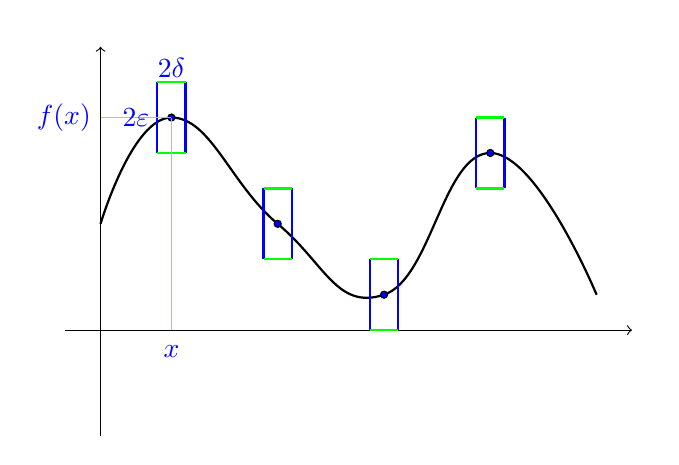
\begin{tikzpicture}[scale=0.9]
        % Draw the coordinate axes
        \draw[->] (-0.5,0) -- (7.5,0) node[right] {};
        \draw[->] (0,-1.5) -- (0,4) node[above] {};
        
        % Draw a smoother continuous curve with local maxima and minima
        \draw[thick] plot[domain=0:7, samples=150, smooth, tension=0.8] 
          coordinates {
            (0,1.5) (1,3) (2.5,1.5) (4,0.5) (5.5,2.5) (7,0.5)
          };
        
        % Mark points on the curve
        \draw[fill=blue] (1,3) circle (0.05);
        \draw[fill=blue] (2.5,1.5) circle (0.05);
        \draw[fill=blue] (4,0.5) circle (0.05);
        \draw[fill=blue] (5.5,2.5) circle (0.05);
        
        % Draw epsilon-delta boxes with blue vertical and green horizontal edges
        % First box (near first maximum)
        \draw[blue, thick] (0.8,2.5) -- (0.8,3.5);
        \draw[blue, thick] (1.2,2.5) -- (1.2,3.5);
        \draw[green, thick] (0.8,2.5) -- (1.2,2.5);
        \draw[green, thick] (0.8,3.5) -- (1.2,3.5);
        
        % Second box (at inflection point)
        \draw[blue, thick] (2.3,1) -- (2.3,2);
        \draw[blue, thick] (2.7,1) -- (2.7,2);
        \draw[green, thick] (2.3,1) -- (2.7,1);
        \draw[green, thick] (2.3,2) -- (2.7,2);
        
        % Third box (at local minimum)
        \draw[blue, thick] (3.8,0) -- (3.8,1);
        \draw[blue, thick] (4.2,0) -- (4.2,1);
        \draw[green, thick] (3.8,0) -- (4.2,0);
        \draw[green, thick] (3.8,1) -- (4.2,1);
        
        % Fourth box (at second maximum)
        \draw[blue, thick] (5.3,2) -- (5.3,3);
        \draw[blue, thick] (5.7,2) -- (5.7,3);
        \draw[green, thick] (5.3,2) -- (5.7,2);
        \draw[green, thick] (5.3,3) -- (5.7,3);
        
        % Add light blue horizontal and vertical guide lines only for the first point
        \draw[blue!30, thin] (1,0) -- (1,3);
        \draw[blue!30, thin] (0,3) -- (1,3);
        
        % Add only one x label on x-axis
        \node[blue] at (1,-0.3) {$x$};
        
        % Add f(x) label
        \node[blue, left] at (0,3) {$f(x)$};
        
        % Add epsilon and delta labels for the first box
        \node[blue] at (0.5,3) {$2\varepsilon$};
        \node[blue] at (1, 3.7) {$2\delta$};
      \end{tikzpicture}
      \caption{Uniform continuity means that the box above does not change dimensions no matter where the point is (hence, the name uniform). }
    \end{subfigure}
    \hfill 
    \begin{subfigure}[b]{0.48\textwidth}
      \centering
      \begin{tikzpicture}[scale=0.9]
        % Draw the coordinate axes
        \draw[->] (-0.5,0) -- (7.5,0) node[right] {};
        \draw[->] (0,-1.5) -- (0,4) node[above] {};
        
        % Draw a smoother, curvy continuous function
        \draw[thick] plot[domain=0:7, samples=300, smooth, tension=0.6] 
          coordinates {
            (0.5,0) (1.2,-0.8) (2,1.5) (3,1) (4,3) (5,2.5) (6,0.5) (6.5,0.8) (7,2)
          };
        
        % Mark points on the curve
        \draw[fill=blue] (0.5,0) circle (0.05);
        \draw[fill=blue] (1.2,-0.8) circle (0.05);
        \draw[fill=blue] (2,1.5) circle (0.05);
        \draw[fill=blue] (4.4,3.06) circle (0.05);
        \draw[fill=blue] (6,0.5) circle (0.05);
        \draw[fill=blue] (7,2) circle (0.05);
        
        % Draw boxes with blue vertical and green horizontal edges in varying dimensions
        % Second box (thin and tall)
        \draw[blue, thick] (1.1,-1.2) -- (1.1,-0.4);
        \draw[blue, thick] (1.3,-1.2) -- (1.3,-0.4);
        \draw[green, thick] (1.1,-1.2) -- (1.3,-1.2);
        \draw[green, thick] (1.1,-0.4) -- (1.3,-0.4);
        
        % Third box (medium rectangle, slightly taller)
        \draw[blue, thick] (1.75,1.3) -- (1.75,1.7);
        \draw[blue, thick] (2.25,1.3) -- (2.25,1.7);
        \draw[green, thick] (1.75,1.3) -- (2.25,1.3);
        \draw[green, thick] (1.75,1.7) -- (2.25,1.7);
        
        % Fourth box (large square) - moved to the right of the peak and down 1 unit
        \draw[blue, thick] (4.4-0.4,2.6) -- (4.4-0.4,3.4);
        \draw[blue, thick] (5.2-0.4,2.6) -- (5.2-0.4,3.4);
        \draw[green, thick] (4.4-0.4,2.6) -- (5.2-0.4,2.6);
        \draw[green, thick] (4.4-0.4,3.4) -- (5.2-0.4,3.4);
        
        % Fifth box (thin and short)
        \draw[blue, thick] (5.9,0.3) -- (5.9,0.7);
        \draw[blue, thick] (6.1,0.3) -- (6.1,0.7);
        \draw[green, thick] (5.9,0.3) -- (6.1,0.3);
        \draw[green, thick] (5.9,0.7) -- (6.1,0.7);
      \end{tikzpicture}
      \caption{In continuity, there are no restrictions on the dimensions of this box. It just has to exist for every point, through a function of $\epsilon$.}
    \end{subfigure}
    \caption{Uniform continuity vs continuity.}
    \label{fig:uniform_vs_regular_continuity}
  \end{figure}

  With this intuition, it is easy to see the result below. 

  \begin{lemma}[Uniform Continuity Implies Continuity]
    If $f$ is uniformly continuous on the set $E$, it is continuous at each point of that set. However, the converse is not generally true. 
  \end{lemma}

  \begin{example}
    Let $f: \mathbb{R} \longrightarrow \mathbb{R}, \; f(x) = 3x+7$. Then $f$ is uniformly continuous. Choose $\epsilon > 0$. Let $\delta = \epsilon / 3$. Choose $x, y \in \mathbb{R}$ and assume $|x-y| < \delta$. Then, 
    \begin{equation}
      | f(x) - f(y) | = | 3x + 7 - 3 y - 7 | = 3 |x-y| < 3 \delta = \epsilon
    \end{equation}
  \end{example}

  \begin{example}
    Let $f: (0, 4) \subset \mathbb{R} \longrightarrow \mathbb{R}, \; f(x) = x^2$. Then $f$ is uniformly continuous on $(0, 4)$. Choose $\epsilon > 0$. Let $\delta = \epsilon / 8$. Choose $x, y \in (0, 4)$ and assume $|x-y| < \delta$. Then, 
    \begin{equation}
      |f(x) - f(y)| = |x^2 - y^2| = (x+y) |x-y| < (4+4) |x-y| = 8\delta = \epsilon
    \end{equation}
  \end{example}

  A natural question one might ask is: under what assumptions is the converse true?  

  \begin{theorem}[Cantor's Theorem on Uniform Continuity]
    A function that is continuous on a compact set is uniformly continuous on that set. 
  \end{theorem}
  \begin{proof}
    
  \end{proof} 

  \begin{theorem}[Uniformly Continuous Function is Linearly Bounded]
    If $f: \mathbb{R} \to \mathbb{R}$ is uniformly continuous, then there exists constants, $a, b \in \mathbb{R}$ such that $|f(x)| \leq a + b|x|$ for all $x \in \mathbb{R}$. 
  \end{theorem}
  \begin{proof}
    Since $f$ is uniformly continuous, for every $\epsilon > 0$ there exists a $\delta > 0$ s.t. 
    \begin{equation}
      |x - y| < \delta \implies |f(x) - f(y)| < \epsilon
    \end{equation}
    for all $x, y \in \mathbb{R}$. Then, setting $y = 0$ and $\epsilon = 1$, we have some $\delta > 0$ s.t. 
    \begin{equation}
      |x| < \delta \implies |f(0) - f(x)| < 1
    \end{equation}
    Now for any $k \in \mathbb{N}$, take $|x| < k \delta$. Then we can construct a sequence $(x_i = i \frac{|x|}{k})_{i = 0}^{k}$, where $x_0 = 0$ and $x_k = |x|$, and from the triangle inequality followed by uniform convergence, we have 
    \begin{equation}
      |x_i - x_{i+1}| = \frac{|x|}{k} < \frac{k\delta}{k} = \delta \implies |f(0) - f(x)| \leq \sum_{i=0}^{k - 1} |f(x_i) - f(x_{i+1})| < \sum_{i=0}^{k-1} 1 = k
    \end{equation} 
    and so we come to the result 
    \begin{equation}
      |x| < k \delta \implies |f(0) - f(x)| < k
    \end{equation}
    Now set $m(x) = \min \{ k \in \mathbb{N} \mid |x| < k \delta \}$. It must be nonempty by the Archimedean property, so it's lower bounded by $1$. 
    \begin{equation}
      |x| < \delta m(x) \implies \frac{|x|}{\delta} < m(x) \implies m(x) \leq \frac{|x|}{\delta} + 1
    \end{equation}
    where the final implication comes from $m(x)$ being minimum. Therefore, 
    \begin{equation}
      |f(x)| \leq |f(0)| + |f(x) - f(0)| \leq |f(0)| + m(x) \leq |f(0)| + \frac{|x|}{\delta} + 1
    \end{equation} 
    and we have found such $a = |f(0)| + 1, b = \frac{1}{\delta}$. 
  \end{proof}

\subsection{Lipshitz and Holder Continuity}

  In both examples, the function satisfied an inequality of form 
  \begin{equation}
    |f(x_1) - f(x_2)| \leq M |x_1 - x_2|
  \end{equation}
  this is called the \textit{Lipshitz inequality}. Lipshitz continuity is a strong form of uniform continuity for functions. Intuitively, a Lipshitz continuous function is limited in how fast it can change (by the Lipshitz constant). 

  \begin{definition}[Lipshitz Continuous Function]
    Given $f: E \subset \mathbb{R} \longrightarrow \mathbb{R}$, $f$ is \textbf{Lipshitz continuous} if there exists a $M > 0$---called the \textit{Lipschitz constant}---such that for all $x, y \in E$, 
    \begin{equation}
      |f(x) - f(y)| \leq M |x - y|
    \end{equation}
  \end{definition}

  Note that Lipshitz continuity pops up as a very natural extension of uniform continuity. The inequality above just means that given an $\epsilon$, we can choose a $\delta$ such that a linear multiple of $\delta$ is always greater than $\epsilon$. This means that Lipshitz continuity is just uniform continuity such that the $\delta$ function is linear:  
  \begin{equation}
    \delta = \delta(\epsilon) = \frac{1}{M} \epsilon
  \end{equation}

  \begin{figure}[H]
    \centering
    \begin{subfigure}[b]{0.32\textwidth}
      \centering
      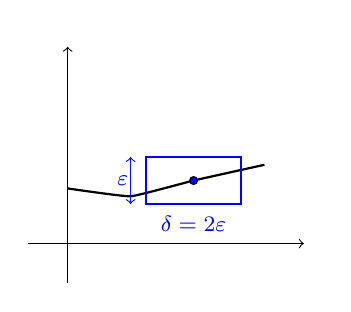
\begin{tikzpicture}[scale=1.0]
        % Draw the axes
        \draw[->] (-0.5,0) -- (3,0) node[right] {};
        \draw[->] (0,-0.5) -- (0,2.5) node[above] {};
        
        % Draw slightly curved function with average slope 1/2
        \draw[thick] plot[domain=0:2.5, smooth, tension=0.2] 
          coordinates {(0,0.7) (0.8,0.6) (1.6,0.8) (2.5,1.0)};
        
        % Mark a point on the curve
        \draw[fill=blue] (1.6,0.8) circle (0.05);
        
        % Draw the epsilon box - wider than tall
        \draw[blue, thick] (1.0,0.5) rectangle (2.2,1.1);
        
        % Add epsilon and delta labels
        \node[blue, font=\footnotesize] at (0.7,0.8) {$\varepsilon$};
        \draw[blue, <->] (0.8,0.5) -- (0.8,1.1);
        
        \node[blue, font=\footnotesize] at (1.6,0.25) {$\delta = 2\varepsilon$};
      \end{tikzpicture}
      \caption{$M = \frac{1}{2}$}
    \end{subfigure}
    \hfill 
    \begin{subfigure}[b]{0.32\textwidth}
      \centering
      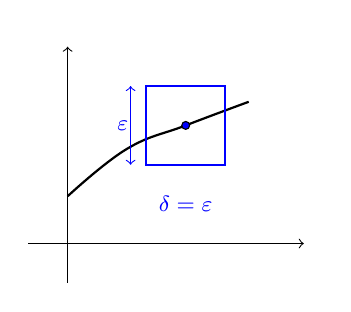
\begin{tikzpicture}[scale=1.0]
        % Draw the axes
        \draw[->] (-0.5,0) -- (3,0) node[right] {};
        \draw[->] (0,-0.5) -- (0,2.5) node[above] {};
        
        % Draw slightly curved function with average slope 1
        \draw[thick] plot[domain=0:2.5, smooth, tension=0.7]
          coordinates {(0,0.6) (0.75,1.2) (1.5,1.5) (2.3,1.8)};
        
        % Mark a point on the curve
        \draw[fill=blue] (1.5,1.5) circle (0.05);
        
        % Draw the epsilon box - square
        \draw[blue, thick] (1.0,1.0) rectangle (2.0,2.0);
        
        % Add epsilon and delta labels
        \node[blue, font=\footnotesize] at (0.7,1.5) {$\varepsilon$};
        \draw[blue, <->] (0.8,1.0) -- (0.8,2.0);
        
        \node[blue, font=\footnotesize] at (1.5,0.5) {$\delta = \varepsilon$};
      \end{tikzpicture}
      \caption{$M = 1$}
    \end{subfigure}
    \hfill 
    \begin{subfigure}[b]{0.32\textwidth}
      \centering
      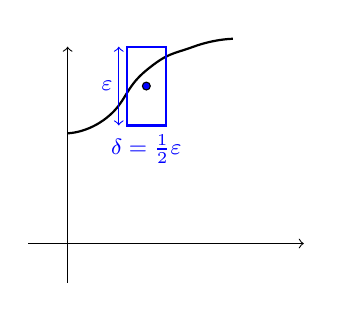
\begin{tikzpicture}[scale=1.0]
        % Draw the axes
        \draw[->] (-0.5,0) -- (3,0) node[right] {};
        \draw[->] (0,-0.5) -- (0,2.5) node[above] {};
        
        % Draw slightly curved function with average slope 2
        \draw[thick] plot[domain=0:1.25, smooth, tension=0.9]
          coordinates {(0,1.4) (0.5,1.6) (1.0,2.2) (1.6,2.5) (2.1, 2.6)};
        
        % Mark a point on the curve
        \draw[fill=blue] (1.0,2.0) circle (0.05);
        
        % Draw the epsilon box - taller than wide
        \draw[blue, thick] (0.75,1.5) rectangle (1.25,2.5);
        
        % Add epsilon and delta labels
        \node[blue, font=\footnotesize] at (0.5,2.0) {$\varepsilon$};
        \draw[blue, <->] (0.65,1.5) -- (0.65,2.5);
        
        \node[blue, font=\footnotesize] at (1.0,1.2) {$\delta = \frac{1}{2}\varepsilon$};
      \end{tikzpicture}
      \caption{$M = 2$}
    \end{subfigure}
    \caption{Relationship between slope $M$ and the ratio of $\delta$ to $\varepsilon$}
    \label{fig:slope-epsilon-delta}
  \end{figure}

  \begin{definition}[Bi-Lipshitz Continuity]
    A function $f: E \subset \mathbb{R}$ is \textbf{Bi-Lipshitz continuous} if there exists constant $M\geq 1$ such that for all real $x, y \in E$, 
    \[ \frac{1}{M} |x - y| \leq |f(x) - f(y)| \leq M |x - y|\]
    It immediately follows that for $x \neq y$, $ |f(x) - f(y)|$ cannot equal $0$, which means that a bilipshitz map is injective. A bilipshitz map is really just Lipshitz map with its inverse also being Lipshitz. 
  \end{definition}

  \begin{theorem}
    A bilipshitz map $f$ is a homeomorphism onto its image. 
  \end{theorem}

  \begin{definition}[Holder Continuity]
    Given $f: E \subset \mathbb{R} \to \mathbb{R}$, $f$ is \textbf{$\alpha$-Holder continuous} if there exists a $C > 0$ such that for all $x, y \in E$, 
    \begin{equation}
      |f(x) - f(y)| \leq M |x - y|^\alpha
    \end{equation}
  \end{definition}

\subsection{Discontinuity}

  If the function $f: E \longrightarrow \mathbb{R}$ is not continuous at a point of $E$, then this point is called a \textbf{point of discontinuity}, or simply a \textbf{discontinuity} of $f$. That is, $a$ is a point of discontinuity of $f$ if for some neighborhood $V(f(a))$ of $f(a)$, there exists no neighborhood of $a$ whose image under the mapping $f$ is contained in $V(f(a))$. There are three types of discontinuities, ranging from least to most extreme.\footnote{Note that strictly speaking, a removable discontinuity is really a discontinuity of first kind, but in this context we distinguish them. } 

  \begin{definition}[Removable Discontinuity]
    A \textbf{removable discontinuity} is characterized by the fact that the limit $\lim_{x \rightarrow a} f(x) = A$ exists, but $A \neq f(a)$. 

    \begin{figure}[H]
      \centering 
      \begin{tikzpicture}[scale=0.9]
        % Draw the coordinate axes
        \draw[->] (-3,0) -- (3,0) node[right] {$x$};
        \draw[->] (0,-1) -- (0,3) node[above] {$y$};
        
        % Draw the function with a removable discontinuity at x=1
        \draw[thick, domain=-2.5:0.95, samples=100, smooth] plot (\x, {(\x*\x - 1)/(\x - 1)});
        \draw[thick, domain=1.05:2.5, samples=100, smooth] plot (\x, {(\x*\x - 1)/(\x - 1)});
        
        % Mark the discontinuity point
        \draw[fill=white] (1,2) circle (0.07);  % Open circle at (1,2)
        
        % Mark the function value at x=1
        \draw[fill=black] (1,1) circle (0.07);  % Filled circle at (1,1)
        
        % Mark the x-axis
        \foreach \x in {-2,-1,1,2}
          \draw (\x,0.1) -- (\x,-0.1) node[below] {$\x$};
        \draw (0,0.1) -- (0,-0.1) node[below] {$0$};
      \end{tikzpicture}
      \caption{A function with a removable discontinuity at $x=1$. The function is defined as $f(x) = \frac{x^2 - 1}{x - 1}$ for $x \neq 1$ and $f(1) = 1$. The limit of the function as $x$ approaches $1$ is $2$ (shown by the open circle), but the function value at $x=1$ is $1$ (shown by the filled circle).}
      \label{fig:removable-discontinuity}
    \end{figure}
  \end{definition}

  This means that we can modify $f$ and define a new function $\Tilde{f}: E \longrightarrow \mathbb{R}$ as
  \begin{equation}
    \Tilde{f}(x) = \begin{cases} f(x), & x \in E \setminus a \\ A, & x = a \end{cases}
  \end{equation}
  which would be continuous on $E$. 

  \begin{definition}[Jump/Step Discontinuity, of First Kind]
    A \textbf{discontinuity of first kind}, also known as a jump/step discontinuity, is characterized by both the left and right-hand limits 
    \begin{equation}
      \lim_{x \rightarrow a-0} f(x) \text{ and } \lim_{x \rightarrow a+0} f(x)
    \end{equation}
    existing, but at least one of them is not equal to the value $f(a)$ that the function assumes at $a$. 

    \begin{figure}[H]
      \centering 
      \begin{tikzpicture}[scale=1.2, y=0.6cm]  % Vertically compressed with y=0.6cm
        % Draw the coordinate axes
        \draw[->] (-3,0) -- (3,0) node[right] {$x$};
        \draw[->] (0,-1) -- (0,4) node[above] {$y$};
        
        % Draw the function with a step discontinuity at x=0
        % Left part of the function
        \draw[thick, domain=-2.5:0, samples=100] plot (\x, {1 + 0.25*\x*\x});
        
        % Right part of the function
        \draw[thick, domain=0:2.5, samples=100] plot (\x, {2 + 0.25*\x*\x});
        
        % Mark the discontinuity points
        \draw[fill=white] (0,1) circle (0.07cm);  % Open circle at (0,1) with absolute size
        \draw[fill=black] (0,2) circle (0.07cm);  % Filled circle at (0,2) with absolute size 
        % Add dashed line to highlight the discontinuity
        \draw[dashed] (0,1) -- (0,2);
        
        % Mark the x-axis
        \foreach \x in {-2,-1,1,2}
          \draw (\x,0.1) -- (\x,-0.1) node[below] {$\x$};
        \draw (0,0.1) -- (0,-0.1) node[below] {$0$};
        
        % Mark the y-axis
        \foreach \y in {1,2,3}
          \draw (0.1,\y) -- (-0.1,\y) node[left] {$\y$};
      \end{tikzpicture}
      \caption{A function with a step discontinuity at $x=0$. The function is defined as $f(x) = 1 + 0.25x^2$ for $x < 0$ and $f(x) = 2 + 0.25x^2$ for $x \geq 0$. The limit from the left $\lim_{x \to 0^-} f(x) = 1$ is shown by the open circle, while the function value at $x=0$ is $f(0) = 2$ shown by the filled circle. The dashed line highlights the jump in value.}
      \label{fig:step-discontinuity}
    \end{figure}
  \end{definition}

  \begin{definition}[Essential Discontinuity, of Second Kind]
    A \textbf{discontinuity of second kind}, also known as an essential discontinuity, is characterized by at least one of the two limits 
    \begin{equation}
      \lim_{x \rightarrow a-0} f(x) \text{ and } \lim_{x \rightarrow a+0} f(x)
    \end{equation}
    not existing. 

    \begin{figure}[H]
      \centering
      \begin{subfigure}[b]{0.48\textwidth}
        \centering
        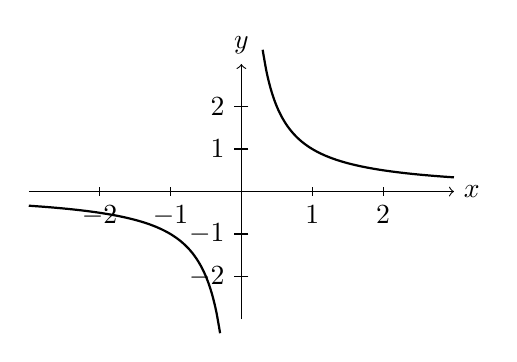
\begin{tikzpicture}[scale=0.9, y=0.6cm]
          % Draw the coordinate axes
          \draw[->] (-3,0) -- (3,0) node[right] {$x$};
          \draw[->] (0,-3) -- (0,3) node[above] {$y$};
          
          % Draw the rational function f(x) = 1/x
          \draw[thick, domain=-3:-0.3, samples=50, smooth] plot (\x, {1/\x});
          \draw[thick, domain=0.3:3, samples=50, smooth] plot (\x, {1/\x});
          
          % Add vertical asymptote at x=0
          \draw[dashed] (0,-3) -- (0,3);
          
          % Mark the x-axis and y-axis
          \foreach \x in {-2,-1,1,2}
            \draw (\x,0.1) -- (\x,-0.1) node[below] {$\x$};
          
          \foreach \y in {-2,-1,1,2}
            \draw (0.1,\y) -- (-0.1,\y) node[left] {$\y$};
        \end{tikzpicture}
        \caption{The function $f(x) = \frac{1}{x}$ has an infinite discontinuity at $x=0$}
        \label{fig:infinite-discontinuity}
      \end{subfigure}
      \hfill 
      \begin{subfigure}[b]{0.48\textwidth}
        \centering
        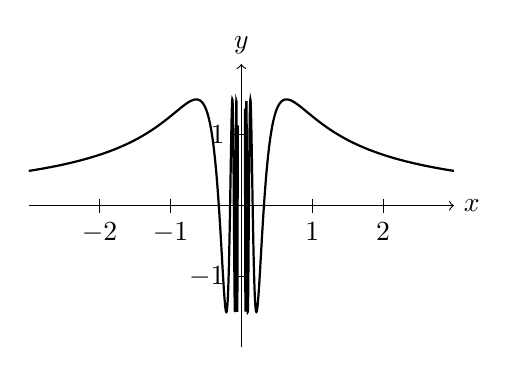
\begin{tikzpicture}[scale=0.9]
          % Draw the coordinate axes
          \draw[->] (-3,0) -- (3,0) node[right] {$x$};
          \draw[->] (0,-2) -- (0,2) node[above] {$y$};
          
          % Draw the function f(x) = sin(1/x)
          \draw[thick, domain=-3:-0.05, samples=800, smooth, variable=\x] 
            plot ({\x}, {sin(1/(-\x) r) * 1.5});
          \draw[thick, domain=0.05:3, samples=800, smooth, variable=\x] 
            plot ({\x}, {sin(1/\x r) * 1.5});
          
          % Add vertical line at x=0
          \draw[dashed] (0,-1.5) -- (0,1.5);
          
          % Mark the x-axis and y-axis
          \foreach \x in {-2,-1,1,2}
            \draw (\x,0.1) -- (\x,-0.1) node[below] {$\x$};
          
          \foreach \y in {-1,1}
            \draw (0.1,\y) -- (-0.1,\y) node[left] {$\y$};
        \end{tikzpicture}
        \caption{The function $f(x) = |1.5 \sin\left(\frac{1}{x}\right)|$ has an oscillatory discontinuity at $x=0$}
        \label{fig:oscillatory-discontinuity}
      \end{subfigure}
      \caption{Examples of discontinuities of the second kind, where the limit does not exist as $x$ approaches the point of discontinuity}
      \label{fig:second-kind-discontinuities}
    \end{figure}
  \end{definition}

  \begin{example}[Dirichlet Function]
    The Dirichlet function, defined
    \begin{equation}
      \mathcal{D}(x) = \begin{cases}
      1, & \text{ if } x \in \mathbb{Q} \\
      0, & \text{ if } x \in \mathbb{R} \setminus \mathbb{Q} 
      \end{cases}
    \end{equation}
    is discontinuous at every point, and obviously all of its discontinuities are of second kind, since in every interval there are both rational and irrational numbers and therefore there exists no limit at any point $a \in \mathbb{R}$. 

    More specifically, given any point $a \in \mathbb{R}$, assume that $a$ is rational. We can set $\epsilon = 0.1$-neighborhood around the value $1$, but no matter how small we let $\delta$, the interval $(a - \delta, a + \delta)$ will contain both rationals and irrationals, meaning that it will map to $\{0,1\}$ always, which is not fully contained in $(0.9, 1.1)$.  
  \end{example}

  Here is a slightly more interesting example. 

  \begin{example}[Riemann Function]
    Let the Riemann function $\mathcal{R}$ be defined
    \begin{equation}
      \mathcal{R}(x) = \begin{cases}
      \frac{1}{n}, & \text{ if } x = \frac{m}{n} \in \mathbb{Q}, \text{ where gcd}(m, n) = 1 \\
      0, & \text{ if } x \in \mathbb{R} \setminus \mathbb{Q}
      \end{cases}
    \end{equation}
    We first note that for any point $a \in \mathbb{R}$, any bounded neighborhood $U(a)$ of it, and any number $N \in \mathbb{N}$, the neighborhood $U(a)$ contains only a finite number of rational numbers $\mathbb{m}{n}$, where $n < N$. By shrinking the neighborhood, we can assume that the denominators of all rational numbers in the neighborhood are larger than $N$, since rationals with larger denominators have smaller gaps between them. Thus, at any point $x \in U(a) \setminus a$, we have 
    \begin{equation}
      \big| \mathcal{R}(x) \big| < \frac{1}{N}
    \end{equation}
    and therefore $\lim_{x \rightarrow a} \mathcal{R} (x) = 0$ at any point $a \in \mathbb{R} \setminus \mathbb{Q}$. Hence, the Riemann function is continuous at any irrational number. 
  \end{example}


